\documentclass[pdflatex,sn-mathphys-num]{sn-jnl}

\usepackage{graphicx}%
\usepackage{multirow}%
\usepackage{amsmath,amssymb,amsfonts}%
\usepackage{amsthm}%
\usepackage{mathrsfs}%
\usepackage[title]{appendix}%
\usepackage{xcolor}%
\usepackage{textcomp}%
\usepackage{manyfoot}%
\usepackage{booktabs}%
\usepackage{algorithm}%
\usepackage{algorithmicx}%
\usepackage{algpseudocode}%
\usepackage{listings}%

\theoremstyle{thmstyleone}
\newtheorem{theorem}{Theorem}
\newtheorem{proposition}[theorem]{Proposition}

\theoremstyle{thmstyletwo}%
\newtheorem{example}{Example}%
\newtheorem{remark}{Remark}%

\theoremstyle{thmstylethree}%
\newtheorem{definition}{Definition}%

\raggedbottom

\begin{document}

\title[PatternGrad: A Local Explanation Method for Noise-Resilient Feature Attribution]{PatternGrad: A Local Explanation Method for Noise-Resilient Feature Attribution in Non-Linear Models}

\author[1]{\fnm{Md Arif Faysal} \sur{Nayem}}

\author*[1]{\fnm{Ohidujjaman} }\email{ohidujjaman@cse.uiu.ac.bd}



\affil*[1]{\orgdiv{Department of Computer Science and Engineering}, \orgname{United International University}, \orgaddress{\street{United City, Madani Avenue}, \city{Dhaka}, \postcode{1212}, \country{Bangladesh}}}
\abstract{In machine learning, suppressor variables are input features that carry no information about the target outcome yet correlate with the noise that corrupts informative features. Conventional local explanation methods often assign false-positive attributions to these variables. Recent pattern-based explanation methods address this issue by converting discriminative explanations into generative signal patterns, but their perturbation-based instantiations rely on randomized perturbation sampling and per-sample surrogate fitting, often over coarse superpixel groupings that limit spatial detail. To overcome these limitations, this paper introduces PatternGrad, a deterministic local explanation method that combines pixel-wise Integrated Gradients with data-adaptive pattern conversion. PatternGrad derives the surrogate analytically, bypassing the perturbation stage entirely, and transforms attributions through the kernel-weighted covariance of the $K$ nearest training neighbors. Evaluated on the XAI-TRIS benchmark across linear, XOR, and rigid-transformation tasks under white and correlated noise, PatternGrad matches or exceeds state-of-the-art perturbation-based pattern conversion in minimizing false-positive attributions (Importance Mass Error) and attains top-tier, best non-filter spatial localization (Earth Mover's Distance) on linear and rigid-transformation tasks, while reducing false-positive attributions below every standard gradient and perturbation baseline on average across the benchmark. Notably, under rigid geometric transformations, PatternGrad maintains accurate spatial localization where conventional explanation methods struggle. On the evaluated benchmark both compared pattern methods operate at native pixel resolution, so the comparison isolates the surrogate and evaluation space rather than the superpixel granularity.}
\keywords{Explainable AI, Feature Attribution, Suppressor Variables, Integrated Gradients, Generative Explanations}

\maketitle

\section{Introduction}\label{sec1}

The rapid deployment of complex, non-linear machine learning models has increased the demand for transparent and accountable decision-making frameworks~\cite{samek2019towards, tjoa2021survey, haufe2024explainable}. Although self-explainable or interpretable architectures, such as prototypical networks and rule-based models, offer built-in explanations, they can compromise predictive accuracy on complex perceptual tasks and may require the model to be retrained from scratch~\cite{rudin2019stop}. Consequently, auditing deployed deep neural networks in practice relies predominantly on post-hoc Explainable Artificial Intelligence (XAI) techniques, which extract feature attributions without modifying the underlying model parameters~\cite{samek2019towards}. Established post-hoc approaches include architecture-specific propagation rules (e.g., LRP~\cite{bach2015pixel} and DeepLIFT~\cite{shrikumar2017learning}), gradient-based sensitivity methods (e.g., Saliency~\cite{simonyan2014deep}, SmoothGrad~\cite{smilkov2017smoothgrad}, and Integrated Gradients~\cite{sundararajan2017}), and model-agnostic local surrogate methods (e.g., LIME~\cite{ribeiro2016} and SHAP~\cite{lundberg2017unified}). Historically, these attribution methods have often been evaluated through anecdotal visual inspection or proxy criteria such as model faithfulness, deletion curves, and perturbation stability~\cite{tjoa2021survey, nauta2023anecdotal}. However, recent studies show that faithfulness to a model's internal computations does not necessarily guarantee a correct explanation: in particular, it does not establish that highlighted features have a genuine statistical dependence on the target outcome~\cite{wilming2022, wilming2023theoretical, haufe2024explainable}.

A critical failure mode of conventional post-hoc XAI arises in the presence of \emph{suppressor variables}: input features that carry no statistical information about the target class on their own but correlate with background noise that corrupts the true signal~\cite{conger1974revised, friedman2005graphical, haufe2014, weichwald2015causal}. To maximize predictive accuracy, discriminative (\emph{backward}) classifiers may assign non-zero weights to these variables to remove correlated noise from informative foreground features~\cite{haufe2014, wilming2022}. Analytical and empirical benchmarks show that widely used gradient-based, propagation-based, and perturbation-based XAI methods can conflate this noise-cancellation role with genuine feature relevance, systematically assigning false-positive attributions to uninformative background regions~\cite{wilming2022, wilming2023theoretical, clark2024, oliveira2024benchmarking}. For linear models, Haufe et al.~\cite{haufe2014} addressed this problem by distinguishing backward discriminative filters from \emph{forward} generative activation patterns. They showed that transforming model weights using the data covariance matrix can suppress contributions from uninformative noise variables. Neural methods such as PatternNet and PatternAttribution~\cite{kindermans2018learning} extend this principle layer by layer, but evaluations on the non-linear XAI-TRIS benchmark indicate that they may fail to suppress false positives under complex non-linear interactions and spatial transformations~\cite{clark2024}. More recently, PatternLocal~\cite{gjoelbye2025} extended forward pattern conversion to non-linear classifiers by fitting a local linear surrogate around each target instance (e.g., using LIME~\cite{ribeiro2016} or GLIME~\cite{tan2023}, a generalized LIME framework with flexible masking and kernel conventions) and regressing the local neighborhood against the surrogate's scalar response. Despite its conceptual appeal, LIME-driven pattern conversion has three practical limitations. First, Monte Carlo perturbation sampling introduces estimation variance into the surrogate weights, which can propagate through the covariance transform, particularly along low-variance noise directions~\cite{haufe2014, wilming2022}. Second, fitting a separate surrogate for each instance using thousands of synthetic perturbations increases computational latency and tuning overhead~\cite{gjoelbye2025}. Third, the use of superpixel masking to keep computation tractable restricts attributions to coarse regions that may cross fine-grained object boundaries~\cite{gjoelbye2025}; in the benchmark configuration reviewed here, the public reference implementation instead runs LIME at native pixel level, so this discretization bottleneck is not itself exercised in our comparisons, which concern the variance, cost, and evaluation space of the surrogate stage. Notably, these bottlenecks originate in the perturbation-based surrogate stage rather than in PatternLocal's covariance conversion itself, which already operates directly on the empirical training manifold over a nearest-neighbor subset with an adaptive locality kernel~\cite{gjoelbye2025}. Thus, deterministic, pixel-level, and computationally scalable local pattern attribution for non-linear models remains an open challenge.

To address this gap, this study aims to remove surrogate-sampling variance, superpixel discretization, and per-instance regression overhead from perturbation-based instantiations of local generative pattern conversion while retaining theoretical guarantees against suppressor-induced false positives. This work introduces \emph{PatternGrad}, a deterministic local explanation framework that combines path-based gradient attribution with on-manifold generative covariance conversion. While retaining the training-anchored generative pattern-conversion principle and the adaptive Gaussian locality kernel of PatternLocal, PatternGrad replaces the stochastic perturbation-based surrogate $\mathbf{w}^{\text{LIME}}$ with the deterministic, axiomatic attribution vector of Integrated Gradients (IG)~\cite{sundararajan2017} evaluated directly in native pixel space. Integrated Gradients satisfies \emph{Completeness} and \emph{Sensitivity} and can mitigate gradient saturation. A kernel-weighted regression of the centered training neighborhood against the analytical surrogate responses, with $\ell_2$-ridge regularization, yields a closed-form transformation. This transformation is evaluated matrix-free using a two-pass matrix--vector product with time and space complexity of $\mathcal{O}(KD)$ beyond a single exact nearest-neighbor search over the training set, leaving the neighborhood size $K$ as the only structural hyperparameter of the conversion stage once the IG surrogate and locality metric are fixed. This paper evaluates PatternGrad across the $54$-configuration evaluation grid of the synthetic XAI-TRIS benchmark~\cite{clark2024}, covering linear (\texttt{LIN}), non-linear exclusive-OR (\texttt{XOR}), and rigid geometric transformation (\texttt{RIGID}) tasks under both uncorrelated (\texttt{WHITE}) and spatially correlated (\texttt{CORR}) background noise. Explanation quality is measured using Earth Mover's Distance (EMD)~\cite{bonneel2011, clark2024} to assess spatial transport accuracy and Importance Mass Error (IME)~\cite{arras2022, clark2024} to quantify false-positive attribution leakage into the background.

PatternGrad offers a fast, reproducible, high-resolution tool for auditing models used in applications such as medical imaging, neuroimaging, and industrial visual inspection. In these settings, correlated sensor noise and physiological background variation can mislead conventional saliency maps~\cite{haufe2014, clark2024, oliveira2024benchmarking}. Across the XAI-TRIS benchmark suites, PatternGrad matches or surpasses state-of-the-art perturbation-based pattern conversion in reducing false-positive attributions (IME) and attains top-tier spatial localization (EMD) on linear and rigid-transformation tasks, while attaining a lower mean false-positive attribution error than every standard gradient and perturbation baseline evaluated in this study. Under position- and orientation-varying rigid transformations (\texttt{RIGID}), PatternGrad preserves accurate pixel-level localization where conventional XAI methods degrade. In the measured pipeline accounting of this paper, PatternGrad's full per-instance cost (surrogate plus covariance conversion) is $0.10$--$0.32$ seconds on a single CPU, faster in every evaluated configuration than the conversion stage alone of surrogate-based pattern conversion ($0.40$--$0.80$ seconds; $1.8\times$--$5.0\times$ per configuration), whose stochastic surrogate front-end lies outside both comparisons (Sect.~\ref{sec:res_runtime}). In terms of operational requirements, PatternGrad needs access to the model's internal gradients and a representative set of training samples. It is therefore unsuitable when a model is available only through an API or when representative training data are scarce~\cite{gjoelbye2025}. The main contributions of this work are as follows:

\begin{itemize}
    \item \textbf{Deterministic, Pixel-Level Pattern Conversion:} This paper introduces a local attribution framework that combines analytical Integrated Gradients with a data-driven covariance transformation based on similar training examples. This avoids randomized perturbation sampling, off-manifold binary-mask reconstructions, and coarse superpixel boundary artifacts.
    \item \textbf{An Efficient Closed-Form Estimator:} This work formulates a matrix-free computational procedure that avoids explicitly constructing large local covariance matrices and eliminates per-instance surrogate optimization. The resulting method requires only a single structural hyperparameter, the neighborhood size, to govern the conversion stage.
    \item \textbf{Comprehensive Empirical Validation and Runtime Acceleration:} Paired evaluations across linear, non-linear, and rigid-transformation tasks on XAI-TRIS demonstrate reduced false-positive attribution leakage and precise spatial localization; under conversion-stage accounting, PatternGrad attains $3.4\times$ to $81.8\times$ (median $9.2\times$) speedups over surrogate-driven pattern conversion, and its full measured pipeline (surrogate plus conversion) is faster than the baseline's conversion stage alone in every evaluated configuration (Sect.~\ref{sec:res_runtime}).
\end{itemize}

\section{Conventional Methods}\label{sec:conventional}

\subsection{Integrated Gradients (IG)}\label{sec:ig}
Standard gradient-based attribution methods quantify feature importance by computing the local partial derivatives of the model prediction $f(\mathbf{x}_\star)$ with respect to the input $\mathbf{x}_\star$. However, raw gradients frequently suffer from \emph{saturation}, where the model output flattens in the vicinity of $\mathbf{x}_\star$, yielding near-zero gradients even for features that strongly contribute to the prediction. To overcome this limitation, Integrated Gradients (IG)~\cite{sundararajan2017} attributes importance by accumulating gradients along a straight-line path from a chosen uninformative reference baseline $\mathbf{r} \in \mathbb{R}^D$ (such as a zero vector) to the target instance $\mathbf{x}_\star$. Formally, the attribution score $s_i^{\text{IG}}(\mathbf{x}_\star)$ for the $i$-th feature is defined as:
\begin{equation}
    s_i^{\text{IG}}(\mathbf{x}_\star) = (x_{\star, i} - r_i) \int_{0}^{1} \frac{\partial f(\mathbf{r} + \gamma(\mathbf{x}_\star - \mathbf{r}))}{\partial x_i} \, d\gamma,
\end{equation}
where $\gamma \in [0, 1]$ parameterizes the linear interpolation path between $\mathbf{r}$ and $\mathbf{x}_\star$. By integrating gradients over the entire path rather than evaluating them solely at $\mathbf{x}_\star$, IG satisfies two fundamental axiomatic properties: \emph{Sensitivity} (guaranteeing non-zero attribution for any single feature that alters the prediction relative to the baseline) and \emph{Completeness}, where the attributions sum to the exact difference in model output, $\sum_{i=1}^D s_i^{\text{IG}}(\mathbf{x}_\star) = f(\mathbf{x}_\star) - f(\mathbf{r})$. In practice, the path integral is efficiently approximated via a Riemann sum over $M$ discrete interpolation steps:
\begin{equation}
    \hat{s}_i^{\text{IG}}(\mathbf{x}_\star) = \frac{x_{\star, i} - r_i}{M} \sum_{m=1}^{M} \frac{\partial f\left(\mathbf{r} + \frac{m}{M}(\mathbf{x}_\star - \mathbf{r})\right)}{\partial x_i}.
\label{eq:ig_riemann}
\end{equation}
a right-endpoint Riemann sum (the quadrature used in all experiments, with nodes $\frac{m}{M}$, $m = 1, \dots, M$, so the target instance $\mathbf{x}_\star$ is included and the baseline $\mathbf{r}$ excluded).


\subsection{Local Interpretable Model-agnostic Explanations (LIME)}
Local Interpretable Model-agnostic Explanations (LIME)~\cite{ribeiro2016} explains an individual prediction $f(\mathbf{x}_\star)$ by approximating the complex model $f$ locally around the target instance $\mathbf{x}_\star$ using an interpretable surrogate model $g \in G$. In its general form, the surrogate is obtained by minimizing $\mathcal{L}(f, g, \Pi_{\mathbf{x}_\star}) + \Omega(g)$, where $\mathcal{L}$ measures local fidelity within a neighborhood around $\mathbf{x}_\star$ weighted by the proximity kernel $\Pi_{\mathbf{x}_\star}$, and $\Omega(g)$ penalizes surrogate complexity. We write the kernel subscript uniformly as $\Pi_{\mathbf{x}_\star}$, indicating proximity to the target instance $\mathbf{x}_\star$; in the simplified representation space, this center corresponds to the interpretable representation of the target, $\mathbf{z}'_\star = h_{\mathbf{x}_\star}(\mathbf{x}_\star) = \mathbf{1}$. 

In standard practice, $g$ is parameterized as a linear model operating in a simplified representation space $\mathcal{Z} \subseteq \mathbb{R}^{D'}$, and $\mathcal{L}$ is defined as the squared loss~\cite{tan2023}. Let $h_{\mathbf{x}_\star}^{-1}: \mathcal{Z} \to \mathcal{X}$ denote the reconstruction mapping that projects a simplified perturbation $\mathbf{z}' \in \mathcal{Z}$ back into the original input space $\mathcal{X}$. LIME estimates a feature-importance vector $\mathbf{w}^{\text{LIME}}$ (together with an intercept $v_0$) via kernel-weighted regularized linear regression over the \emph{perturbation-space} kernel $\Pi^{\text{LIME}}_{\mathbf{x}_\star}$, which we use to distinguish it from the training-manifold locality kernel of Sect.~\ref{sec:patternlocal}:
\begin{equation}
    \mathbf{s}^{\text{LIME}}(\mathbf{x}_\star) = \mathbf{w}^{\text{LIME}} = \operatorname*{argmin}_{v_0,\, \mathbf{v}} \; \mathbb{E}_{\mathbf{z}'} \big[ \Pi^{\text{LIME}}_{\mathbf{x}_\star}(\mathbf{z}') \left( f(h_{\mathbf{x}_\star}^{-1}(\mathbf{z}')) - v_0 - \mathbf{v}^\top \mathbf{z}' \right)^2 \big] + \lambda R(\mathbf{v}),
    \label{eq:lime}
\end{equation}
where $R(\mathbf{v})$ is a regularization penalty weighted by $\lambda$; centering the design matrix at its kernel-weighted mean absorbs $v_0$ and yields an equivalent intercept-free formulation in the covariance-ratio form of Eq.~\eqref{eq:pl_closed} below. For image data, $\mathbf{z}' \sim \operatorname{Uni}(\{0, 1\}^{D'})$ represents a binary mask over $D'$ superpixels, $\Pi^{\text{LIME}}_{\mathbf{x}_\star}(\mathbf{z}') = \exp(-\|\mathbf{z}'_\star - \mathbf{z}'\|_2^2 / \sigma_L^2)$ is an exponential locality kernel measuring the squared Euclidean distance of the simplified representation $\mathbf{z}'$ to the target's representation $\mathbf{z}'_\star = \mathbf{1}$ (for binary masks, this coincides with the Hamming distance, i.e., the number of masked superpixels), and $R(\mathbf{v}) = \|\mathbf{v}\|_2^2$ corresponds to ridge regularization. Perturbed inputs are reconstructed via $h_{\mathbf{x}_\star}^{-1}(\mathbf{z}') = \mathbf{x}_\star \odot B(\mathbf{z}') + \mathbf{r} \odot (\mathbf{1} - B(\mathbf{z}'))$, where $B: \{0, 1\}^{D'} \to \{0, 1\}^D$ broadcasts each binary superpixel indicator $z'_j$ to its constituent pixels, $\odot$ denotes the element-wise product, and $\mathbf{r}$ is the same uninformative reference baseline as in the IG formulation (Sect.~\ref{sec:ig}). Because $\mathbf{w}^{\text{LIME}}$ acts as a local discriminative filter to fit $f$, it remains susceptible to assigning non-zero importance to correlated suppressor variables~\cite{wilming2022}.


\subsection{PatternLocal}\label{sec:patternlocal}
Standard local linear explanation methods (such as LIME~\cite{ribeiro2016}, KernelSHAP~\cite{lundberg2017unified}, and local gradients) approximate a complex model $f$ around an instance of interest $\mathbf{x}_\star$ using a linear surrogate weight vector $\mathbf{w}$. However, as discriminative filter parameters, $\mathbf{w}$ often assigns non-zero weights to suppressor variables in order to cancel out correlated background noise. To mitigate these false-positive attributions, PatternLocal~\cite{gjoelbye2025} converts the local surrogate weights $\mathbf{w}$ into a generative, data-driven \emph{pattern} $\mathbf{a}$ that reflects only statistically relevant signal features.

Let $h_{\mathbf{x}_\star}: \mathcal{X} \to \mathbb{R}^{D'}$ denote a simplified local input representation around $\mathbf{x}_\star$: for superpixel-based surrogates, $h_{\mathbf{x}_\star}(\mathbf{x})$ aggregates the image $\mathbf{x}$ over the $D'$ superpixels of the segmentation anchored at $\mathbf{x}_\star$ (one scalar per superpixel, such as its mean intensity), so it is defined for \emph{arbitrary} inputs, including the training samples; in the pixel-level regime of this work $h_{\mathbf{x}_\star} \equiv \mathrm{id}$ and $D' = D$. The pattern $\mathbf{a} \in \mathbb{R}^{D'}$ obtained in the superpixel case is mapped back to input space by broadcasting each coefficient $a_j$ over the pixels of superpixel $j$ (the adjoint of $h_{\mathbf{x}_\star}$), so the final attribution remains a $D$-dimensional map. Rather than treating the surrogate weights $\mathbf{w}$ directly as the explanation, PatternLocal estimates the attribution pattern $\mathbf{a}$ by regressing the local surrogate response back onto the simplified input features within a kernel-weighted neighborhood $\Pi_{\mathbf{x}_\star}$. Centering the features at their $\Pi_{\mathbf{x}_\star}$-weighted mean $\boldsymbol{\mu}$ absorbs the intercept, so that with the centered representation $\tilde{\mathbf{x}} \mathrel{:=} h_{\mathbf{x}_\star}(\mathbf{x}) - \boldsymbol{\mu}$ and the centered response $\tilde{y} \mathrel{:=} \mathbf{w}^\top \tilde{\mathbf{x}}$, the conversion solves
\begin{equation}
    \mathbf{s}^{\text{PatternLocal}}(\mathbf{x}_\star) = \mathbf{a} = \operatorname*{argmin}_{\mathbf{u}} \; \mathbb{E}_{\mathbf{x} \sim \mathbb{P}_{\mathcal{X}}} \left[ \Pi_{\mathbf{x}_\star}(h_{\mathbf{x}_\star}(\mathbf{x})) \left\| \tilde{\mathbf{x}} - \mathbf{u}\,\tilde{y} \right\|_2^2 \right] + \lambda Q(\mathbf{u}),
    \label{eq:pl_objective}
\end{equation}
where $Q(\mathbf{u})$ is a regularization penalty weighted by $\lambda$ to ensure estimation stability in high-dimensional or sparse neighborhoods. When $Q(\mathbf{u}) = \|\mathbf{u}\|_1$, Eq.~\eqref{eq:pl_objective} corresponds to a kernel-weighted Lasso regression. Under $\ell_2$ regularization ($Q(\mathbf{u}) = \|\mathbf{u}\|_2^2$), the kernel-weighted normal equations of the centered objective admit the exact closed-form solution:
\begin{equation}
    \mathbf{a}_{\ell_2} = \frac{\operatorname{Cov}_{\Pi_{\mathbf{x}_\star}}[h_{\mathbf{x}_\star}(\mathbf{x}), \tilde{y}]}{\operatorname{Var}_{\Pi_{\mathbf{x}_\star}}[\tilde{y}] + \lambda}.
    \label{eq:pl_closed}
\end{equation}
By expressing feature importance as the localized covariance between the input features and the surrogate output $\tilde{y}$ (rather than the true label $y$), PatternLocal preserves both model faithfulness and local fidelity while effectively driving the attribution of uncorrelated suppressor variables to zero.

\section{Proposed Method}\label{sec:proposed}

\subsection{PatternGrad}
The explanation quality of the pattern-conversion paradigm underlying PatternLocal~\cite{gjoelbye2025} rests on two core components: (i) the local surrogate weights $\mathbf{w}$, which compress the local behavior of the model $f$ around a target instance $\mathbf{x}_\star$ into a scalar response $\tilde{y}$, and (ii) the kernel-weighted neighborhood $\Pi_{\mathbf{x}_\star}$ over which the covariance between input features and $\tilde{y}$ is estimated. PatternLocal is formulated for general local linear surrogates, including LIME, KernelSHAP, and local gradients, and, unlike the perturbation stage, its covariance conversion is already computed on the empirical training manifold over a nearest-neighbor subset with an adaptive Gaussian bandwidth~\cite{gjoelbye2025}. The practical limitations targeted in this work therefore arise specifically in its perturbation-based surrogate instantiations rather than in the covariance conversion stage itself. When the surrogate is LIME (Eq.~\eqref{eq:lime}), the weights are estimated via Monte Carlo regression over $N_{\mathcal{L}}$ random input perturbations~\cite{ribeiro2016,tan2023}, introducing estimation variance that scales with the dimensionality of the simplified representation and diminishes only with a large perturbation budget. Moreover, for image data, mask-based surrogates typically operate on $D'$ superpixels rather than individual pixels, constraining the resulting attribution map to be piecewise constant at a granularity coarser than the input space; on the XAI-TRIS configuration reviewed here, however, LIME is instantiated at pixel level ($D' = D = 4{,}096$; Sect.~\ref{sec:param_config}), so superpixel discretization is not the operative difference in our comparison, and with $N_{\mathcal{L}} = 2{,}000$ perturbations against $D' = 4{,}096$ candidate features each per-instance fit is strongly under-determined, a regime in which the ridge penalty and the locality kernel carry the identification. This estimation noise propagates directly into the covariance transform of Eq.~\eqref{eq:pl_closed}, degrading performance precisely where pattern conversion is most needed: because suppressor variables couple with the prediction target through low-variance, noise-carrying directions of the input space~\cite{haufe2014,wilming2022}, a noisy surrogate fit can spuriously latch onto background features.

To eliminate surrogate sampling variance entirely, this work proposes \emph{PatternGrad}. While retaining the training-anchored generative pattern-conversion principle and the adaptive Gaussian locality kernel of PatternLocal, PatternGrad replaces the stochastic perturbation-based surrogate $\mathbf{w}^{\text{LIME}}$ with the deterministic, axiomatic attribution vector of Integrated Gradients (IG), evaluated directly in native pixel space rather than over synthetic binary masks. Because the surrogate is obtained analytically at the target instance, no perturbation stage is required at any point in the pipeline: given $(f, \mathbf{x}_\star, M, K, \lambda, \mathcal{D}_{\text{train}})$, the resulting estimator is completely deterministic, requiring no random mask generation, no out-of-distribution input reconstruction, and no per-instance surrogate optimization. Within the generalized local explanation framework of Tan et al.~\cite{tan2023}, PatternGrad represents the limiting case combining an analytical gradient surrogate with an on-manifold data kernel.

\subsubsection{Analytical Surrogate via Integrated Gradients}\label{sec:pg_surrogate}
PatternGrad instantiates the local surrogate weight vector $\mathbf{w}^{\text{PG}} \in \mathbb{R}^D$ directly as the $M$-step Integrated Gradients attribution vector of Sect.~\ref{sec:conventional}:
\begin{equation}
    \mathbf{w}^{\text{PG}} \mathrel{:=} \hat{\mathbf{s}}^{\text{IG}}(\mathbf{x}_\star),
    \label{eq:pg_surrogate}
\end{equation}
computed via Eq.~\eqref{eq:ig_riemann} along the straight-line path from the uninformative reference baseline $\mathbf{r} = \mathbf{0}$ to $\mathbf{x}_\star$, where $f(\mathbf{x})$ denotes the target class logit. Three methodological properties motivate this choice over a perturbation-based surrogate. First, IG satisfies the fundamental axioms of \emph{Sensitivity} and \emph{Completeness}, and its path integral resolves the local gradient saturation that compromises raw input gradients~\cite{sundararajan2017}. Second, and central to our design, $\mathbf{w}^{\text{PG}}$ is \emph{deterministic}: because no stochastic perturbations of the input enter its computation, the surrogate carries zero Monte Carlo variance (up to the deterministic quadrature error of the $M$-step Riemann sum). Third, the surrogate operates directly in native pixel space ($h_{\mathbf{x}_\star} \equiv \mathrm{id}$ with $D' = D$), avoiding synthetic binary masks altogether; mask-based surrogates reconstruct perturbed inputs off the data manifold through $h_{\mathbf{x}_\star}^{-1}(\mathbf{z}')$, and superpixel-based variants additionally constrain the attribution map to be piecewise constant at a granularity coarser than the input space.

A methodological clarification is in order regarding the role of $\mathbf{w}^{\text{PG}}$ in the conversion stage. Writing $\bar{\mathbf{g}}(\mathbf{x}_\star) \mathrel{:=} \frac{1}{M}\sum_{m=1}^{M} \nabla_{\mathbf{x}} f\!\left(\mathbf{r} + \frac{m}{M}(\mathbf{x}_\star - \mathbf{r})\right)$ for the path-averaged gradient, Eq.~\eqref{eq:ig_riemann} gives $\hat{\mathbf{s}}^{\text{IG}}(\mathbf{x}_\star) = (\mathbf{x}_\star - \mathbf{r}) \odot \bar{\mathbf{g}}(\mathbf{x}_\star)$: an \emph{instance-scaled attribution} whose components carry units of the model output $f$ (slope times input displacement), whereas the local linear slope of $f$ in continuous pixel space is $\bar{\mathbf{g}}(\mathbf{x}_\star)$ itself, with units of $\partial f / \partial x_i$. In mask-based surrogates such as LIME (Eq.~\eqref{eq:lime}), the surrogate slope $\mathbf{w}^{\text{LIME}}$ is defined over dimensionless binary indicators $\mathbf{z}' \in \{0, 1\}^{D'}$ in which toggling a superpixel from $0$ to $1$ moves the input by the displacement $\mathbf{x}_\star - \mathbf{r}$ restricted to that superpixel, so the feature displacement is already absorbed by the interpretable representation and the conversion stage regresses the corresponding continuous feature representations (the aggregated per-superpixel features $h_{\mathbf{x}_\star}(\mathbf{x})$, or the pixel values themselves when $D' = D$) onto $\tilde{y}$, rather than the binary perturbation masks $\mathbf{z}'$. In native pixel space no such representation exists, and PatternGrad deliberately adopts the instance-scaled attribution as the surrogate response generator (Sect.~\ref{sec:pg_covariance}): the response $\tilde{y}^{(j)} = (\mathbf{w}^{\text{PG}})^\top \tilde{\mathbf{x}}^{(j)} = \bar{\mathbf{g}}(\mathbf{x}_\star)^\top \operatorname{diag}(\mathbf{x}_\star - \mathbf{r})\, \tilde{\mathbf{x}}^{(j)}$ applies a diagonal instance-displacement weighting to the neighbor displacements on top of the local slope, so each coordinate contributes its slope component $w^{\text{PG}}_i = (x_{\star,i} - r_i)\,\bar{g}_i$ multiplied by the neighbor's displacement $\tilde{x}^{(j)}_i$. This is not a first-order expansion of $f$ in instance-normalized coordinates $u_i = x_i / (x_{\star,i} - r_i)$, which would instead carry scaled displacements $\tilde{x}_{i} / (x_{\star,i} - r_i)$; $\tilde{y}$ is a genuine model-output response carrying units of the output $f$, and it changes sign in coordinates whose target displacement $(x_{\star,i} - r_i)$ is negative. This instance gating is an intentional design choice: features whose displacement vanishes at the target ($x_{\star,i} = r_i$) are excluded from the surrogate response regardless of their local sensitivity, so the covariance projection concentrates on the coordinates that carry the target's class evidence, and by \emph{Completeness} (up to the Riemann quadrature error) the surrogate satisfies $\mathbf{1}^\top \hat{\mathbf{s}}^{\text{IG}}(\mathbf{x}_\star) = \bar{\mathbf{g}}(\mathbf{x}_\star)^\top (\mathbf{x}_\star - \mathbf{r}) = f(\mathbf{x}_\star) - f(\mathbf{r})$, keeping $\tilde{y}$ commensurate with the model-output contrast between target and baseline. The price of this gating, namely the sign reversal of the local sensitivity for features whose target displacement is negative (as occurs in the negative-polarity shapes of the \texttt{XOR} task) and the residual suppressor response it leaves on canonical linear models relative to the unscaled slope, is analyzed in Remark~\ref{rem:scaling} and quantified empirically in Sect.~\ref{sec:res_ablation}.

\subsubsection{Covariance Conversion on the Training Neighborhood}\label{sec:pg_covariance}
Rather than regressing $\tilde{y}$ onto synthetic binary masks drawn from an artificial perturbation distribution, PatternGrad estimates the forward generative pattern over the empirical data distribution. For a target instance $\mathbf{x}_\star$, let $\mathcal{N}_K(\mathbf{x}_\star) \subset \mathcal{D}_{\text{train}}$ denote the index set of its $K$ nearest training samples under the Euclidean metric. This work defines the normalized, training-anchored locality kernel $\Pi^K_{\mathbf{x}_\star}$ via the weights:
\begin{equation}
    \pi_j = \frac{\mathbf{1}\!\left[j \in \mathcal{N}_K(\mathbf{x}_\star)\right] \, K_\sigma\!\left(\left\|\mathbf{x}^{(j)} - \mathbf{x}_\star\right\|_2\right)}{\sum_{\ell \in \mathcal{N}_K(\mathbf{x}_\star)} K_\sigma\!\left(\left\|\mathbf{x}^{(\ell)} - \mathbf{x}_\star\right\|_2\right)}, \qquad K_\sigma(d) = \exp\!\left(-\frac{d^2}{2\sigma^2}\right),
    \label{eq:pg_kernel}
\end{equation}
where the kernel bandwidth $\sigma \mathrel{:=} \operatorname{median}\{\Vert\mathbf{x}^{(j)} - \mathbf{x}_\star\Vert_2 : j \in \mathcal{N}_K(\mathbf{x}_\star)\}$ is adapted automatically per instance, introducing no additional bandwidth hyperparameter. 

PatternGrad recovers the attribution pattern $\mathbf{a} \in \mathbb{R}^D$ via kernel-weighted ridge regression of the neighborhood inputs onto the surrogate response. Centering at the kernel-weighted neighborhood mean $\boldsymbol{\mu} \mathrel{:=} \sum_{j \in \mathcal{N}_K(\mathbf{x}_\star)} \pi_j \mathbf{x}^{(j)}$ absorbs the intercept: with centered neighbors $\tilde{\mathbf{x}}^{(j)} = \mathbf{x}^{(j)} - \boldsymbol{\mu}$ and centered surrogate responses $\tilde{y}^{(j)} = (\mathbf{w}^{\text{PG}})^\top \tilde{\mathbf{x}}^{(j)}$ (Lines 4--5 of Algorithm~\ref{algo:patterngrad}), the intercept-free conversion solves
\begin{equation}
    \mathbf{a} = \operatorname*{argmin}_{\mathbf{u}} \; \sum_{j \in \mathcal{N}_K(\mathbf{x}_\star)} \pi_j \left\| \tilde{\mathbf{x}}^{(j)} - \mathbf{u}\, \tilde{y}^{(j)} \right\|_2^2 + \lambda \left\| \mathbf{u} \right\|_2^2.
    \label{eq:pg_objective}
\end{equation}
Introducing the local empirical covariance matrix $\mathbf{C}_K \mathrel{:=} \sum_{j \in \mathcal{N}_K(\mathbf{x}_\star)} \pi_j \tilde{\mathbf{x}}^{(j)} \tilde{\mathbf{x}}^{(j)\top}$ and noting that $\operatorname{Cov}_{\Pi^K_{\mathbf{x}_\star}}[\mathbf{x}, \tilde{y}] = \mathbf{C}_K \mathbf{w}^{\text{PG}}$ and $\operatorname{Var}_{\Pi^K_{\mathbf{x}_\star}}[\tilde{y}] = (\mathbf{w}^{\text{PG}})^\top \mathbf{C}_K \mathbf{w}^{\text{PG}}$, the normal equations of Eq.~\eqref{eq:pg_objective} admit the exact closed-form solution:
\begin{equation}
    \mathbf{a} = \frac{\operatorname{Cov}_{\Pi^K_{\mathbf{x}_\star}}\!\left[\mathbf{x},\, \tilde{y}\right]}{\operatorname{Var}_{\Pi^K_{\mathbf{x}_\star}}[\tilde{y}] + \lambda} = \frac{\mathbf{C}_K\, \mathbf{w}^{\text{PG}}}{(\mathbf{w}^{\text{PG}})^\top \mathbf{C}_K \mathbf{w}^{\text{PG}} + \lambda}.
    \label{eq:pg_closed}
\end{equation}

The centering in Eq.~\eqref{eq:pg_objective} is not a cosmetic choice: differentiating the corresponding \emph{uncentered} objective $\sum_j \pi_j \|\mathbf{x}^{(j)} - \mathbf{u}\,(\mathbf{w}^{\text{PG}})^\top \mathbf{x}^{(j)}\|_2^2 + \lambda\|\mathbf{u}\|_2^2$ would return the second-moment ratio $\frac{(\mathbf{C}_K + \boldsymbol{\mu}\boldsymbol{\mu}^\top)\,\mathbf{w}^{\text{PG}}}{(\mathbf{w}^{\text{PG}})^\top (\mathbf{C}_K + \boldsymbol{\mu}\boldsymbol{\mu}^\top)\,\mathbf{w}^{\text{PG}} + \lambda}$, which differs from Eq.~\eqref{eq:pg_closed} whenever $\boldsymbol{\mu} \neq \mathbf{0}$. The centered formulation is the intercept-free ridge estimator actually evaluated in Algorithm~\ref{algo:patterngrad}, and it is the form whose kernel-weighted normal equations coincide with the covariance ratio of Eq.~\eqref{eq:pg_closed}.

Equation~\eqref{eq:pg_closed} transforms the discriminative IG vector $\mathbf{w}^{\text{PG}}$ into its corresponding Haufe-type generative pattern~\cite{haufe2014} localized on the data manifold. Crucially, the $D \times D$ matrix $\mathbf{C}_K$ is never explicitly materialized in memory: stacking the centered neighbors into $\tilde{\mathbf{X}}_K \in \mathbb{R}^{K \times D}$, the numerator $\mathbf{C}_K \mathbf{w}^{\text{PG}}$ is evaluated via the two-pass matrix--vector product $\tilde{\mathbf{X}}_K^\top \big(\boldsymbol{\pi} \odot (\tilde{\mathbf{X}}_K \mathbf{w}^{\text{PG}})\big)$ in $\mathcal{O}(KD)$ time and space. Furthermore, because attribution maps are evaluated after magnitude normalization, the strictly positive scalar denominator $(\mathbf{w}^{\text{PG}})^\top \mathbf{C}_K \mathbf{w}^{\text{PG}} + \lambda$ affects only the global scale of $\mathbf{a}$ and not its spatial direction. Consequently, $\lambda > 0$ serves purely as a numerical stabilization constant, leaving the neighborhood size $K$ as the single structural hyperparameter of the covariance conversion step (for a fixed IG surrogate $(M, \mathbf{r})$ and Euclidean locality kernel) governing the bias--variance trade-off between local fidelity and covariance estimation stability.

\subsubsection{Theoretical Properties}
Because PatternGrad filters the surrogate vector through the local data covariance $\mathbf{C}_K$, its attributions are governed by how input features co-vary with the surrogate response across the local manifold rather than by the discriminative weights alone. The following proposition formalizes how this mechanism suppresses false-positive attributions on uninformative background features. Its premises are generative rather than algebraic: they posit a local signal-plus-noise structure and a denoising property of the surrogate response, and the cancellation is derived from them.

\begin{proposition}[Suppressor cancellation]\label{prop:suppression}
Let $\mathcal{S} \subseteq \mathbb{R}^{D}$ denote the local class-informative signal subspace around $\mathbf{x}_\star$, let $P_{\mathcal{N}} = \mathbf{I}_D - P_{\mathcal{S}}$ denote the orthogonal projector onto its complementary noise subspace, and suppose the neighborhood inputs follow the local generative model $\mathbf{x} = \mathbf{s} + \boldsymbol{\eta}$ with class signal $\mathbf{s} \in \mathcal{S}$ and noise $\boldsymbol{\eta}$ spanning both $\mathcal{S}$ and $\mathcal{N}$ (so that $\mathbf{C}_K$ is in general \emph{not} block-diagonal between the two subspaces, $P_{\mathcal{N}}\mathbf{C}_K P_{\mathcal{S}} \neq \mathbf{0}$), where the signal is uncorrelated with the noise-subspace coordinates of the input, $\operatorname{Cov}_{\Pi^K_{\mathbf{x}_\star}}[\mathbf{s}, P_{\mathcal{N}}\mathbf{x}] = \mathbf{0}$. Suppose further that the centered surrogate response is a linear denoised signal estimate: there exist a linear functional $\psi$ on $\mathcal{S}$ and a residual $\varepsilon$ with $\operatorname{Cov}_{\Pi^K_{\mathbf{x}_\star}}[P_{\mathcal{N}}\mathbf{x}, \varepsilon] = 0$ such that $\tilde{y} = \psi(\mathbf{s}) + \varepsilon$. Then, even if the discriminative surrogate assigns non-zero weights to suppressor directions in the noise subspace ($P_{\mathcal{N}}\mathbf{w}^{\text{PG}} \neq \mathbf{0}$), PatternGrad assigns zero attribution to the noise subspace: $P_{\mathcal{N}}\mathbf{a} = \mathbf{0}$. The statement concerns the population conversion; with the empirical estimator of Eq.~\eqref{eq:pg_closed} over $K$ neighbors, $P_{\mathcal{N}}\mathbf{a}$ instead vanishes up to sampling fluctuation of order $\mathcal{O}_p(K^{-1/2})$.
\end{proposition}

\begin{proof}
By Eq.~\eqref{eq:pg_closed}, $\mathbf{a} = \mathbf{C}_K\mathbf{w}^{\text{PG}} / c$ with $c = (\mathbf{w}^{\text{PG}})^\top \mathbf{C}_K \mathbf{w}^{\text{PG}} + \lambda > 0$, so by linearity of the covariance in its first argument,
\begin{equation*}
    P_{\mathcal{N}}\mathbf{a} = \frac{P_{\mathcal{N}}\operatorname{Cov}_{\Pi^K_{\mathbf{x}_\star}}[\mathbf{x}, \tilde{y}]}{c} = \frac{\operatorname{Cov}_{\Pi^K_{\mathbf{x}_\star}}[P_{\mathcal{N}}\mathbf{x}, \tilde{y}]}{c}.
\end{equation*}
The numerator is genuinely at stake: decomposing $\mathbf{w}^{\text{PG}} = P_{\mathcal{S}}\mathbf{w}^{\text{PG}} + P_{\mathcal{N}}\mathbf{w}^{\text{PG}}$ gives
\begin{equation*}
    P_{\mathcal{N}}\mathbf{C}_K\mathbf{w}^{\text{PG}} = P_{\mathcal{N}}\mathbf{C}_K P_{\mathcal{S}}\mathbf{w}^{\text{PG}} + P_{\mathcal{N}}\mathbf{C}_K P_{\mathcal{N}}\mathbf{w}^{\text{PG}},
\end{equation*}
and under correlated noise neither term vanishes individually, since $P_{\mathcal{N}}\mathbf{C}_K P_{\mathcal{S}} \neq \mathbf{0}$ by hypothesis and $P_{\mathcal{N}}\mathbf{w}^{\text{PG}} \neq \mathbf{0}$ by supposition. The cancellation therefore cannot be read off block-diagonality; it follows from the generative premises. By linearity of the covariance in its second argument, $\operatorname{Cov}_{\Pi^K_{\mathbf{x}_\star}}[P_{\mathcal{N}}\mathbf{x}, \tilde{y}] = \operatorname{Cov}_{\Pi^K_{\mathbf{x}_\star}}[P_{\mathcal{N}}\mathbf{x}, \psi(\mathbf{s})] + \operatorname{Cov}_{\Pi^K_{\mathbf{x}_\star}}[P_{\mathcal{N}}\mathbf{x}, \varepsilon]$. The first term vanishes because $\psi(\mathbf{s})$ is a function of $\mathbf{s} \in \mathcal{S}$ alone and $\operatorname{Cov}_{\Pi^K_{\mathbf{x}_\star}}[\mathbf{s}, P_{\mathcal{N}}\mathbf{x}] = \mathbf{0}$ by hypothesis; the second vanishes by the denoising property of $\varepsilon$. Hence the numerator is $\mathbf{0}$ and, since $c > 0$ for any $\lambda > 0$, $P_{\mathcal{N}}\mathbf{a} = \mathbf{0}$.
\end{proof}

Two remarks locate the substantive content of the premises. First, Proposition~\ref{prop:suppression} is stated for a \emph{general} surrogate response: the denoising premise involves only $\psi$ and $\varepsilon$, not the specific definition of the surrogate weights $\mathbf{w}$, so the result applies verbatim to any local linear surrogate, including a LIME regression. The premise must nonetheless be assessed per surrogate choice. On the canonical two-variable suppressor model of Remark~\ref{rem:scaling}, the \emph{unscaled} slope $\mathbf{w} = \boldsymbol{\beta} = (1, -1)^\top$ satisfies it exactly, since $\tilde{y} = \boldsymbol{\beta}^\top \tilde{\mathbf{x}} = \tilde{S}$ is a pure signal estimate with $\varepsilon = \mathbf{0}$; the instance-scaled surrogate $\mathbf{w}^{\text{PG}} = \mathbf{x}_\star \odot \boldsymbol{\beta}$ instead produces the residual $\varepsilon = s_\star \tilde{N}$ on the noise coordinate, for which $\operatorname{Cov}[P_{\mathcal{N}}\mathbf{x}, \varepsilon] = s_\star \neq 0$ unless $s_\star = 0$, so the premise (and with it exact cancellation) holds for $\mathbf{w}^{\text{PG}}$ only in the uniform-displacement regime, where $x_{\star,i} - r_i$ is constant across the coupled coordinates and the scaling reduces to a global constant multiplying $\boldsymbol{\beta}$ (Remark~\ref{rem:scaling}). Second, the cancellation is stated at the population level of the kernel-weighted neighborhood: at finite $K$, $\mathbf{C}_K$ is an empirical covariance estimated from $K$ neighbors, so $P_{\mathcal{N}}\mathbf{a}$ vanishes only up to sampling fluctuation of order $\mathcal{O}_p(K^{-1/2})$, which declines as the neighborhood grows (Proposition~\ref{prop:consistency}, Remark~\ref{rem:adaptivelimit}) and is not separately controlled by $\lambda$.

Proposition~\ref{prop:suppression} delineates the mechanism by which PatternGrad counteracts the suppressor vulnerability of discriminative attributions~\cite{haufe2014, wilming2022}. A local discriminative filter $\mathbf{w}$, whether fitted via LIME regression or accumulated via backpropagation, is free to exploit background directions that cancel correlated noise in order to sharpen its prediction, yielding $w_i \neq 0$ for suppressor features $i \notin \mathcal{F}^+$ (where $\mathcal{F}^+ \subseteq \{1, \dots, D\}$ denotes the ground-truth informative feature support, defined per scenario in Sect.~\ref{sec:dataset}). In the correlated-noise (\texttt{CORR}) scenarios of the XAI-TRIS benchmark~\cite{clark2024}, spatially smoothed background noise induces clusters of such suppressor pixels, causing gradient-based attribution maps to bleed outside the ground-truth support. PatternGrad, in contrast, weights every surrogate component by its generative covariance with the local input statistics: the coordinate $a_i$ represents the expected change in feature $i$ implied by a unit change in the surrogate response $\tilde{y}$ across the training manifold around $\mathbf{x}_\star$. Because suppressor cancellations in the noise subspace yield vanishing net covariance with the denoised surrogate response $\tilde{y}$, their pattern coefficients are attenuated toward zero as characterized by Proposition~\ref{prop:suppression}.

\begin{remark}[Instance-scaled versus unscaled surrogates]\label{rem:scaling}
The instance scaling in Eq.~\eqref{eq:pg_surrogate} is not neutral for exact suppressor cancellation. Consider the canonical two-variable linear suppressor model $X_1 = S + N$ (informative signal plus noise) and $X_2 = N$ (uninformative suppressor), with independent $S, N \sim \mathcal{N}(0,1)$, input covariance $\boldsymbol{\Sigma} = \left(\begin{smallmatrix} 2 & 1 \\ 1 & 1 \end{smallmatrix}\right)$, and Bayes-optimal linear score $f(\mathbf{x}) = x_1 - x_2$ with filter $\boldsymbol{\beta} = (1, -1)^\top$. For a strictly linear $f$, the path-averaged gradient equals the filter, $\bar{\mathbf{g}} = \boldsymbol{\beta}$, and the population transform of the \emph{unscaled slope} recovers the exact Haufe forward pattern, $\boldsymbol{\Sigma}\,\boldsymbol{\beta} = (1, 0)^\top$, which assigns strictly zero attribution to the suppressor $X_2$. The instance-scaled surrogate of Eq.~\eqref{eq:pg_surrogate} instead gives $\mathbf{w}^{\text{PG}} = \mathbf{x}_\star \odot \boldsymbol{\beta} = (s_\star + n_\star,\, -n_\star)^\top$ at $\mathbf{x}_\star = (s_\star + n_\star,\, n_\star)^\top$, and
\begin{equation*}
    \boldsymbol{\Sigma}\,\mathbf{w}^{\text{PG}} = \left(\begin{smallmatrix} 2 & 1 \\ 1 & 1 \end{smallmatrix}\right) \left(\begin{smallmatrix} s_\star + n_\star \\ -n_\star \end{smallmatrix}\right) = \left(\begin{smallmatrix} 2 s_\star + n_\star \\ s_\star \end{smallmatrix}\right),
\end{equation*}
which retains a suppressor component proportional to the target's signal amplitude $s_\star$: pre-multiplying by $(\mathbf{x}_\star - \mathbf{r})$ re-weights the columns of $\boldsymbol{\Sigma}$ (and, locally, of $\mathbf{C}_K$) instance-dependently, breaking the exact noise-cancellation balance $\operatorname{Cov}(X_2, \boldsymbol{\beta}^\top \mathbf{x}) = 0$. In addition, any informative feature with $x_{\star,i} = r_i$ is gated out of the surrogate response even when $\bar{g}_i \neq 0$, and negative displacements flip the sign of the local sensitivity before projection. PatternGrad nevertheless adopts the scaled attribution deliberately (Sect.~\ref{sec:pg_surrogate}): it trades the exact asymptotic cancellation enjoyed by the unscaled slope for per-instance selectivity, concentrating the surrogate response on the target's active support. This trade-off is quantified empirically by the PG-Grad ablation: for strictly linear $f$ the pointwise gradient coincides with $\bar{\mathbf{g}}$, so there the ablation isolates the scaling choice, whereas for non-linear $f$ it additionally replaces path integration with the pointwise gradient, partially confounding the two design axes (Sect.~\ref{sec:res_ablation}). The fully integrated but unscaled surrogate $\bar{\mathbf{g}}(\mathbf{x}_\star)$, optionally rescaled after conversion as $(\mathbf{x}_\star - \mathbf{r}) \odot \mathbf{a}$, is a natural complementary variant left for future work.
\end{remark}

A second property characterizes the asymptotic population limit of the estimator under a stylized uniform weighting; the limit under the actual adaptive kernel of Eq.~\eqref{eq:pg_kernel} is addressed in Remark~\ref{rem:adaptivelimit} below.

\begin{proposition}[Consistency under uniform weights]\label{prop:consistency}
Fix $f$, $\mathbf{x}_\star$, $\mathbf{r}$, $M$, and $\lambda > 0$, and assume $\mathcal{D}_{\text{train}}$ consists of $N$ i.i.d.\ draws from $\mathbb{P}_{\mathcal{X}}$ with finite second moments. In the global limit $K = N$ under uniform kernel weights $\pi_j = 1/N$, as $N \to \infty$ the PatternGrad estimator converges in probability to the population Haufe transform:
\begin{equation}
    \mathbf{a}^{\infty} = \frac{\boldsymbol{\Sigma}\, \mathbf{w}^{\text{PG}}}{(\mathbf{w}^{\text{PG}})^\top \boldsymbol{\Sigma}\, \mathbf{w}^{\text{PG}} + \lambda}, \qquad \boldsymbol{\Sigma} \mathrel{:=} \operatorname{Cov}_{\mathbb{P}_{\mathcal{X}}}[\mathbf{x}].
    \label{eq:pg_limit}
\end{equation}
The ridge constant $\lambda > 0$ is retained in the denominator throughout; the unregularized population Haufe pattern is recovered as the additional limit $\lambda \to 0$.
\end{proposition}

\begin{proof}
Under uniform weights $\pi_j = 1/N$, the matrix $\mathbf{C}_N$ in Eq.~\eqref{eq:pg_closed} reduces to the empirical sample covariance over $\mathcal{D}_{\text{train}}$. By the Weak Law of Large Numbers for i.i.d.\ samples, the first and second empirical moments converge in probability to their population counterparts, yielding $\mathbf{C}_N \xrightarrow{p} \boldsymbol{\Sigma}$ as $N \to \infty$. Because the closed-form expression of Eq.~\eqref{eq:pg_closed} is a continuous function of $\mathbf{C}_N$ on the domain $(\mathbf{w}^{\text{PG}})^\top \mathbf{C}_N\, \mathbf{w}^{\text{PG}} + \lambda > 0$ (guaranteed by $\lambda > 0$), the result follows by the Continuous Mapping Theorem.
\end{proof}

\begin{remark}[Limit under the adaptive median-bandwidth kernel]\label{rem:adaptivelimit}
Proposition~\ref{prop:consistency} is stated under explicit uniform weighting and should be read as a stylized population benchmark rather than as the limit of Algorithm~\ref{algo:patterngrad} itself. Under the adaptive kernel of Eq.~\eqref{eq:pg_kernel}, setting $K = N$ does not produce uniform weights: the bandwidth $\sigma = \operatorname{median}\{\|\mathbf{x}^{(j)} - \mathbf{x}_\star\|_2 : j \in \mathcal{N}_K(\mathbf{x}_\star)\}$ converges in probability to the finite population median distance $\sigma_\infty(\mathbf{x}_\star) < \infty$ from $\mathbf{x}_\star$ to $\mathbb{P}_{\mathcal{X}}$, so the Gaussian weights $K_\sigma(d_j) = \exp(-d_j^2 / 2\sigma^2)$ remain strictly non-uniform at $K = N$ (assigning unnormalized weight $1$ at $d_j = 0$ and $\exp(-1/2) \approx 0.606$ at the median distance). In this regime, $\mathbf{C}_N$ converges in probability not to the unweighted population covariance $\boldsymbol{\Sigma}$, but to an $\mathbf{x}_\star$-anchored, Gaussian-weighted population covariance,
\begin{equation*}
    \mathbf{C}_N \xrightarrow{p} \boldsymbol{\Sigma}_\infty(\mathbf{x}_\star) \mathrel{:=} \frac{\mathbb{E}_{\mathbb{P}_{\mathcal{X}}}\!\left[\, w_\infty(d)\, (\mathbf{x} - \boldsymbol{\mu}_\infty)(\mathbf{x} - \boldsymbol{\mu}_\infty)^\top \right]}{\mathbb{E}_{\mathbb{P}_{\mathcal{X}}}[w_\infty(d)]}, \quad \boldsymbol{\mu}_\infty \mathrel{:=} \frac{\mathbb{E}_{\mathbb{P}_{\mathcal{X}}}[w_\infty(d)\,\mathbf{x}]}{\mathbb{E}_{\mathbb{P}_{\mathcal{X}}}[w_\infty(d)]},
\end{equation*}
with $w_\infty(d) = \exp(-d^2 / 2\sigma_\infty^2)$ and $d = \|\mathbf{x} - \mathbf{x}_\star\|_2$, and the corresponding pattern is a locally Gaussian-weighted Haufe-type conversion anchored at $\mathbf{x}_\star$. Recovering the unweighted population covariance $\boldsymbol{\Sigma}$ of Eq.~\eqref{eq:pg_limit} additionally requires the flat-kernel limit $\sigma \to \infty$, under which $w_\infty \equiv 1$, $\boldsymbol{\mu}_\infty \to \mathbb{E}_{\mathbb{P}_{\mathcal{X}}}[\mathbf{x}]$, and $\boldsymbol{\Sigma}_\infty \to \boldsymbol{\Sigma}$; equivalently, Eq.~\eqref{eq:pg_kernel} could be replaced by uniform weights whenever $K = N$.
\end{remark}

Taken together, Proposition~\ref{prop:consistency} and Remark~\ref{rem:adaptivelimit} show that the neighborhood size $K$ smoothly interpolates between a purely local manifold covariance estimate around $\mathbf{x}_\star$ and a globally supported, $\mathbf{x}_\star$-anchored population conversion under the adaptive kernel of Eq.~\eqref{eq:pg_kernel}; the unweighted population Haufe conversion~\cite{haufe2014} of the IG statistic is obtained in the additional flat-kernel limit $\sigma \to \infty$ (or by uniform weights at $K = N$). Intermediate $K$ is selected via validation data. Computationally, the per-instance cost comprises $M$ backward passes of complexity $\mathcal{O}(M C_{\text{back}})$ for the IG surrogate, where $C_{\text{back}}$ denotes the cost of a single backward pass, an exact Euclidean $K$-nearest-neighbor search over $\mathcal{D}_{\text{train}}$ of complexity $\mathcal{O}(ND)$ (or $\mathcal{O}(ND + N \log K)$ with heap-based partial selection), and the $\mathcal{O}(KD)$ matrix-free two-pass product of Eq.~\eqref{eq:pg_closed}, which is dominated by the retrieval term whenever $K \ll N$; the overall per-instance complexity is therefore $\mathcal{O}(ND + M C_{\text{back}} + KD)$. Relative to LIME-driven PatternLocal, the random perturbation sampling and per-instance surrogate regression are eliminated and the surrogate cost matches standard IG; the retrieval term is a single pass over the pre-stored training matrix, computed once per instance and shared across methods, and lies outside the conversion-stage timings reported in Sect.~\ref{sec:res_runtime}. Algorithm~\ref{algo:patterngrad} summarizes the complete procedure.

\begin{algorithm}[t]
\caption{PatternGrad Attribution}\label{algo:patterngrad}
\begin{algorithmic}[1]
\Require Differentiable classifier $f$, target instance $\mathbf{x}_\star \in \mathbb{R}^D$, training set $\mathcal{D}_{\text{train}}$, uninformative reference baseline $\mathbf{r} \in \mathbb{R}^D$ (default $\mathbf{r} = \mathbf{0}$), quadrature steps $M$, neighborhood size $K$, ridge constant $\lambda > 0$
\Ensure Attribution map $\mathbf{a} \in \mathbb{R}^D$
\State $\mathbf{w}^{\text{PG}} \leftarrow \frac{1}{M} \sum_{m=1}^{M} \nabla_{\mathbf{x}} f\!\left(\mathbf{r} + \frac{m}{M}\, (\mathbf{x}_\star - \mathbf{r})\right) \odot (\mathbf{x}_\star - \mathbf{r})$ \Comment{Analytical IG surrogate, Eq.~\eqref{eq:pg_surrogate}; $\mathbf{r} = \mathbf{0}$ in all experiments}
\State Retrieve the $K$ nearest neighbors $\mathcal{N}_K(\mathbf{x}_\star) \subset \mathcal{D}_{\text{train}}$ of $\mathbf{x}_\star$ and locally re-index them as $j, \ell \in \{1, \dots, K\}$ \Comment{Eq.~\eqref{eq:pg_kernel} indexes over $\mathcal{D}_{\text{train}}$ with $\pi_j = 0$ for $j \notin \mathcal{N}_K(\mathbf{x}_\star)$}
\State Compute bandwidth $\sigma \leftarrow \operatorname{median}_{j} \left\|\mathbf{x}^{(j)} - \mathbf{x}_\star\right\|_2$ and kernel weights $\boldsymbol{\pi} \in \mathbb{R}^K$ via Eq.~\eqref{eq:pg_kernel}; precompute the weighted neighborhood mean $\boldsymbol{\mu} \leftarrow \sum_{\ell=1}^{K} \pi_\ell\, \mathbf{x}^{(\ell)}$
\State Form centered neighborhood matrix $\tilde{\mathbf{X}}_K \in \mathbb{R}^{K \times D}$ with rows $\tilde{\mathbf{x}}^{(j)} \leftarrow \mathbf{x}^{(j)} - \boldsymbol{\mu}$, $j = 1, \dots, K$
\State $\tilde{\mathbf{y}} \leftarrow \tilde{\mathbf{X}}_K \mathbf{w}^{\text{PG}}$ \Comment{Centered surrogate responses}
\State $\mathbf{a} \leftarrow \tilde{\mathbf{X}}_K^\top (\boldsymbol{\pi} \odot \tilde{\mathbf{y}}) \,\big/\, \big(\tilde{\mathbf{y}}^\top (\boldsymbol{\pi} \odot \tilde{\mathbf{y}}) + \lambda\big)$ \Comment{Matrix-free evaluation of Eq.~\eqref{eq:pg_closed}}
\State \Return $\mathbf{a}$
\end{algorithmic}
\end{algorithm}


\section{Experiments}

\subsection{Dataset: XAI-TRIS Benchmark}\label{sec:dataset}
The proposed method is evaluated on XAI-TRIS, a synthetic benchmark introduced by Clark et al.~\cite{clark2024} to assess explanation faithfulness in the presence of suppressor variables. Each scenario--$\alpha$ configuration consists of $N = 40{,}000$ grayscale images of size $64 \times 64$ ($D = 4{,}096$ features), denoted by $\mathcal{D} = \{(\mathbf{x}^{(n)}, y^{(n)})\}_{n=1}^{N}$, with balanced binary labels drawn according to $y^{(n)} \sim \operatorname{Bernoulli}(1/2)$.

Each instance $\mathbf{x}^{(n)} \in \mathbb{R}^{D}$ is constructed by additively combining a class-dependent foreground signal $\mathbf{a}^{(n)} \in \mathbb{R}^{D}$ with a background noise vector $\boldsymbol{\eta}^{(n)} \sim \mathcal{N}(\mathbf{0}, \mathbf{I}_{D})$:
\begin{equation}
    \mathbf{x}^{(n)} = \alpha R^{(n)}\!\left(H\!\left(\mathbf{a}^{(n)}\right)\right) + (1-\alpha)G\!\left(\boldsymbol{\eta}^{(n)}\right),
    \label{eq:xaitris_generation}
\end{equation}
where the transformed signal and noise components are each Frobenius-normalized (Euclidean norm scaled to $1$) prior to the convex combination; no further rescaling is applied, and since the combined image has Euclidean norm at most $1$, its pixel values lie in $[-1, 1]^{D}$. The signal-to-noise ratio (SNR) parameter is swept across nine discrete levels, $\alpha \in \{0.1, 0.2, \dots, 0.9\}$. Here, $H$ denotes a two-dimensional Gaussian spatial smoothing filter ($\sigma_{\text{smooth}} = 1.5$) followed by a relative maximum-support threshold that zeroes smoothed coefficients below $5\%$ of the largest coefficient, so the foreground edges blend into the background; $R^{(n)}$ applies a scenario-specific spatial transformation; and $G$ governs the background noise structure ($G = \mathrm{id}$ under \texttt{WHITE}; a two-dimensional Gaussian spatial filter with $\sigma_{\text{smooth}} = 10$ under \texttt{CORR}). The ground-truth support $\mathcal{F}^+$ is defined as the non-zero support of the smoothed, thresholded foreground $\alpha R^{(n)}(H(\mathbf{a}^{(n)}))$, i.e., after smoothing and the $5\%$-of-peak cutoff, not the raw tetromino silhouette; for \texttt{LIN} it is the union of the T- and L-shape supports.

Two background noise regimes are evaluated:
\begin{itemize}
    \item \textbf{White noise (WHITE):} $G$ is the identity operator, yielding standard independent Gaussian noise.
    \item \textbf{Correlated noise (CORR):} $G$ is a two-dimensional Gaussian spatial filter with $\sigma_{\text{smooth}} = 10$. This spatial smoothing induces \emph{suppressor variables}, background pixels outside the foreground support that carry no direct class information, but correlate with the noise corrupting the foreground pattern. Predictive models can exploit these pixels to denoise the foreground signal, frequently causing discriminative attribution methods to assign spurious importance to background regions~\cite{haufe2014, wilming2022}.
\end{itemize}

Figure~\ref{fig:dataset} illustrates the generated data under the two noise regimes at $\alpha = 0.2$: for each foreground task and each class, the MASK columns show the signed class-conditional foreground signal (the Gaussian-smoothed tetromino pattern before binarization; in \texttt{LIN} this is the class's own tetromino, T for $y = 0$ and L for $y = 1$) and the INST. columns the corresponding $64 \times 64$ instance (Fig.~\ref{fig:dataset}: \texttt{WHITE} left, \texttt{CORR} right). The MASK panels therefore visualize the per-class signal rather than the binary evaluation mask $\mathcal{F}^+$: in \texttt{LIN}, $\mathcal{F}^+$ comprises the union of both tetromino regions for either class, since the absence of one pattern is as informative as the presence of the other. Under WHITE, the tetromino signal competes only with independent pixel-level noise, whereas under CORR the signal is partially absorbed into smooth, spatially extended perturbation blobs that give the background its suppressor structure.

\begin{figure}[t]
\centering
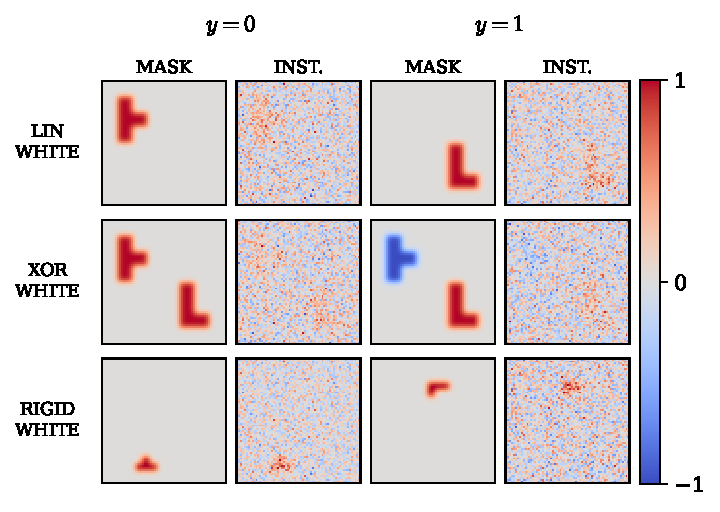
\includegraphics[width=0.495\textwidth]{fig_dataset_white.pdf}\hfill
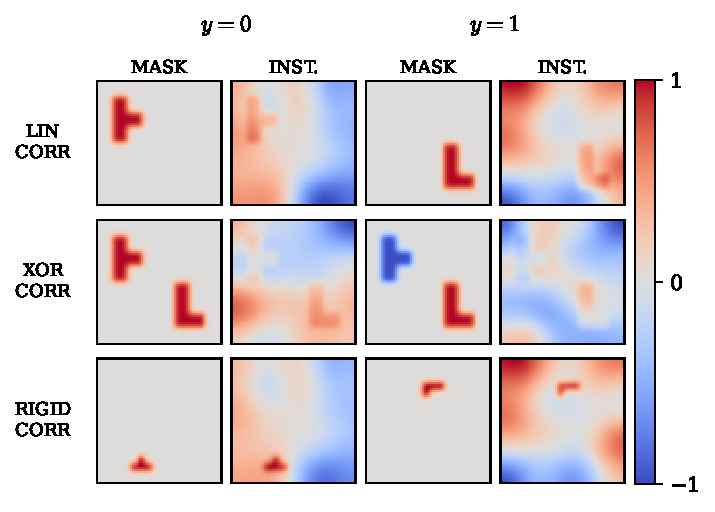
\includegraphics[width=0.495\textwidth]{fig_dataset_corr.pdf}
\caption{Example instances of the XAI-TRIS benchmark at $\alpha = 0.2$ under white noise (\textbf{left}, \texttt{WHITE}) and correlated noise (\textbf{right}, \texttt{CORR}). For each foreground task (\texttt{LIN}, \texttt{XOR}, \texttt{RIGID}) and each class $y \in \{0, 1\}$, the MASK columns show the signed class-conditional foreground signal (the Gaussian-smoothed tetromino pattern before binarization; in \texttt{LIN} this is the class's own tetromino, T for $y = 0$ and L for $y = 1$) and the INST. columns show the corresponding instance, formed by combining the foreground signal with the background noise (Eq.~\eqref{eq:xaitris_generation}). The MASK panels visualize the per-class signal, not the binary evaluation mask $\mathcal{F}^+$ used for the EMD/IME metrics, which is class-independent: in \texttt{LIN} it comprises the union of both tetromino regions (Sect.~\ref{sec:dataset}). Under \texttt{WHITE} the background is independent pixel-level noise; under \texttt{CORR} the spatially smoothed background ($\sigma_{\text{smooth}} = 10$) forms smooth blue/red perturbation blobs that induce \emph{suppressor variables}, background pixels that carry no direct class information but correlate with the noise corrupting the foreground signal. In \texttt{RIGID}, the active tetromino is randomly translated and rotated.}
\label{fig:dataset}
\end{figure}

Across both noise regimes, the foreground signal $\mathbf{a}^{(n)}$ is constructed from `T'-shaped ($\mathbf{a}^{\text{T}}$) and `L'-shaped ($\mathbf{a}^{\text{L}}$) tetrominoes under three classification tasks:
\begin{itemize}
    \item \textbf{Linear (LIN):} $R^{(n)}$ is the identity transformation. Class $y = 0$ is indicated by a `T'-shaped tetromino near the upper-left corner, whereas class $y = 1$ is indicated by an `L'-shaped tetromino near the lower-right corner.
    \item \textbf{Exclusive-OR (XOR):} $R^{(n)}$ is the identity transformation, and both tetrominoes appear simultaneously in every image. For $y = 0$, the two shapes share the same polarity ($\mathbf{a}^{\text{T}} + \mathbf{a}^{\text{L}}$ or $-\mathbf{a}^{\text{T}} - \mathbf{a}^{\text{L}}$), whereas for $y = 1$, they carry opposite polarities ($\mathbf{a}^{\text{T}} - \mathbf{a}^{\text{L}}$ or $-\mathbf{a}^{\text{T}} + \mathbf{a}^{\text{L}}$).
    \item \textbf{Rigid-body transformation (RIGID):} Following the class encoding of the LIN scenario, $R^{(n)}$ applies a random spatial translation and $90^\circ$-increment rotation to the active tetromino, introducing position and orientation variance.
\end{itemize}

Combining the three foreground tasks with the two background noise conditions yields six benchmark suites: \texttt{LIN-WHITE}, \texttt{LIN-CORR}, \texttt{XOR-WHITE}, \texttt{XOR-CORR}, \texttt{RIGID-WHITE}, and \texttt{RIGID-CORR}. The original benchmark additionally defines a multiplicative scenario (\texttt{MULT}), in which the noise modulates the foreground signal multiplicatively~\cite{clark2024}; \texttt{MULT} is omitted from the present evaluation because the covariance-based pattern conversion underlying both PatternLocal and PatternGrad presupposes the additive signal-plus-noise generative structure of Sect.~\ref{sec:proposed}, so the multiplicative regime lies outside the scope of the conversion and is left for future work. The ground-truth feature mask $\mathcal{F}^{+}(\mathbf{x}^{(n)})$ comprises all pixels within the active tetromino support. In the static \texttt{LIN} scenario, both the $\mathbf{a}^{\text{T}}$ and $\mathbf{a}^{\text{L}}$ regions are included in $\mathcal{F}^{+}$, as the absence of one pattern is as informative as the presence of the other. Each dataset is partitioned into training ($\mathcal{D}_{\text{train}}$), validation ($\mathcal{D}_{\text{val}}$), and test ($\mathcal{D}_{\text{test}}$) subsets using a 90/5/5 split.

\subsection{Experimental Protocol and Baselines}\label{sec:param_config}

\subsubsection{Classifier Training and Accuracy Gating}\label{sec:protocol_training}
For each of the $54$ $(\text{scenario}, \alpha)$ configurations, a multilayer perceptron (MLP) classifier is trained on $\mathcal{D}_{\text{train}}$. The network consists of four hidden layers with widths $128$, $64$, $32$, and $16$, each formed by a linear layer followed by batch normalization, a ReLU activation, and dropout with rate $0.25$, and a final linear layer producing two output logits (input dimension $D = 4{,}096$). Training uses the Adam optimizer (learning rate $10^{-4}$, batch size $128$) with a ReduceLROnPlateau scheduler (monitoring validation accuracy, factor $0.1$, patience $100$) for a maximum of $500$ epochs, and early stopping with a patience of $100$ epochs monitors the validation loss on $\mathcal{D}_{\text{val}}$, retaining the model checkpoint with the minimum validation loss. At explanation time the network is evaluated in inference mode (using the running batch-normalization statistics and disabling dropout), so the classifier $f$ entering all attribution methods is a fixed deterministic function.

To ensure that attribution scores reflect meaningful model abstractions rather than uninformative decision boundaries of an underfitted classifier, a strict $90\%$ test-accuracy gate is enforced. Any configuration in which the trained MLP achieves less than $90\%$ classification accuracy on $\mathcal{D}_{\text{test}}$ is documented and excluded from attribution scoring (Sect.~\ref{sec:results}). For all configurations passing this threshold, explanations are generated for $600$ correctly classified instances drawn from $\mathcal{D}_{\text{test}}$, of which $30$ are reserved for per-configuration hyperparameter tuning and the remaining $570$ are scored (Sect.~\ref{sec:hyper}). All compared methods are evaluated on the exact same held-out test instances to guarantee strictly paired comparisons, and all resulting attribution maps are magnitude-normalized prior to metric evaluation.

\subsubsection{Evaluated Methods and Parameter Configuration}
PatternGrad is evaluated alongside an ablation variant and a suite of established baselines:
\begin{itemize}
    \item \textbf{PatternGrad and Ablation:} PatternGrad (\texttt{analytical\_ig}) computes the analytical Integrated Gradients (IG) surrogate $\mathbf{w}^{\text{PG}} = \hat{\mathbf{s}}^{\text{IG}}(\mathbf{x}_\star)$ using $M = 50$ quadrature steps from a zero baseline $\mathbf{r} = \mathbf{0}$ (Eq.~\eqref{eq:ig_riemann}). Next, the $K$ nearest training neighbors of $\mathbf{x}_\star$ in $\mathcal{D}_{\text{train}}$ are retrieved under the Euclidean metric, and adaptive Gaussian kernel weights $\boldsymbol{\pi}$ are assigned using the per-instance median neighbor distance $\sigma = \operatorname{median}\{\Vert{}\mathbf{x}^{(j)} - \mathbf{x}_\star\Vert{}_2 : \mathbf{x}^{(j)} \in \mathcal{N}_K(\mathbf{x}_\star)\}$ (Eq.~\eqref{eq:pg_kernel}). The closed-form $\ell_2$-ridge pattern (Eq.~\eqref{eq:pg_closed}, $\lambda = 10^{-5}$) is then evaluated via the matrix-free product $\tilde{\mathbf{X}}_K^{\top}(\boldsymbol{\pi} \odot (\tilde{\mathbf{X}}_K \mathbf{w}^{\text{PG}}))$. To probe the surrogate design space, an \texttt{analytical\_grad} ablation (PG-Grad) is also evaluated by substituting the raw input gradient $\mathbf{w}^{\text{PG}} = \nabla_{\mathbf{x}} f(\mathbf{x}_\star)$, the unscaled pointwise local slope, into the identical covariance-conversion pipeline (Remark~\ref{rem:scaling}).
    \item \textbf{Local Surrogate and Pattern Baselines:} LIME~\cite{ribeiro2016} is instantiated at pixel level, following the configuration of the public PatternLocal reference implementation on XAI-TRIS~\cite{gjoelbye2025}: the surrogate operates on $D' = D = 4{,}096$ per-pixel binary masks (no superpixel segmentation) reconstructed against the zero reference $\mathbf{r} = \mathbf{0}$, with $N_{\mathcal{L}} = 2{,}000$ sampled masks per instance, an exponential locality kernel $\exp(-\|\mathbf{z}'_\star - \mathbf{z}'\|_2^2 / \sigma_L^2)$ whose bandwidth $\sigma_L$ is tuned per configuration (Sect.~\ref{sec:param_config}; selected $30.0$ in 40 of the 47 configurations, $10$--$20$ in the remaining low-SNR \texttt{CORR} points), and weighted ridge regression with $\lambda_L = 1$ (fitted by the centered Woodbury solver, intercept included). PatternLocal~\cite{gjoelbye2025} converts the fitted LIME weights into a generative pattern via the closed-form kernel-weighted ridge estimator (Eq.~\eqref{eq:pl_closed}, $\lambda = 10^{-5}$, zero covariance shrinkage) using a Gaussian locality kernel with adaptive median bandwidth and neighborhood ratio $k_{\text{ratio}} \in \{0.05, 0.5, 1.0\}$ tuned per configuration on the same tuning subset.
    \item \textbf{Gradient and Edge-Detection Baselines:} Unconverted discriminative baselines include the raw Input Gradient, reported as Saliency in the tables and figures, Integrated Gradients ($M = 50$, $\mathbf{r} = \mathbf{0}$), and SmoothGrad ($M = 50$ samples with additive Gaussian noise of standard deviation $\sigma_{\text{SG}} = 0.1 \times (\max \mathbf{x} - \min \mathbf{x})$ of the explained instance). In addition, Sobel and Laplace filters are included as model-independent spatial edge baselines.
\end{itemize}

In total, thirteen method entries are computed, twelve of which are distinct after magnitude normalization; all rank statements in this paper refer to the twelve distinct entries, counting Saliency and Input Gradient once: PatternGrad (analytical IG surrogate, $M = 50$, $\mathbf{r} = \mathbf{0}$); its PG-Grad ablation (raw input gradient surrogate, identical pipeline); LIME-driven PatternLocal ($\lambda = 10^{-5}$, zero shrinkage, adaptive median bandwidth, tuned $k_{\text{ratio}}$); LIME (pixel-level, $N_{\mathcal{L}} = 2{,}000$, tuned $\sigma_L$, $\lambda_L = 1$); the raw Input Gradient; the Saliency baseline (the magnitude map of the Input Gradient, numerically identical to it after magnitude normalization and reported under the same entry); the unconverted Integrated Gradients map ($M = 50$, $\mathbf{r} = \mathbf{0}$); the unconverted SmoothGrad map ($M = 50$, $\sigma_{\text{SG}}$ as above); DeepLIFT (Rescale rule, zero reference); GradientSHAP ($50$ stochastic references drawn as zero plus Gaussian noise of standard deviation $0.1 \times (\max \mathbf{x} - \min \mathbf{x})$); GuidedBackprop (ReLU-guided backpropagation); and the Sobel and Laplace edge filters. All methods receive the identical magnitude-normalized scoring protocol of Sect.~\ref{sec:eval_metrics}. The main figures (Figs.~\ref{fig:emd_curves} and \ref{fig:ime_curves}) display the ten methods that define the main comparison; the PG-Grad ablation and DeepLIFT are reported in Table~\ref{tab:headline} and analyzed in Sect.~\ref{sec:res_ablation}.

\noindent\textbf{Baseline selection and omissions.} Several methods discussed in Sects.~\ref{sec1} and \ref{sec:conventional} are deliberately excluded. First, PatternNet and PatternAttribution~\cite{kindermans2018learning} and LRP~\cite{bach2015pixel} are deterministic pattern-conversion and propagation methods that, like PatternGrad, require no per-instance surrogate fitting. They are omitted because their behavior on this benchmark has already been characterized by Clark et al.~\cite{clark2024}, who find that PatternNet and PatternAttribution recover the signal optimally on the linear XAI-TRIS tasks in the presence of suppressor variables but fail to fully suppress false-positive attributions under the non-linear XOR and rigid-transformation tasks (on which such neural pattern and propagation methods conflate noise cancellation with feature relevance). Re-evaluating them under this paper's protocol would not, moreover, be paired-comparable: the attribution outcomes depend on the specific trained classifier checkpoints, which differ between training runs, and Clark et al.'s quantitative results were produced under their own checkpoints and budget. Re-running them would therefore duplicate, under a different training seed, the qualitative picture already published, rather than inform the hypothesis tested here, namely whether replacing the stochastic surrogate of the strongest available conversion baseline with an analytical path-integrated vector changes the outcome. Their reported weakness nonetheless motivates our comparison against the unconverted discriminative and edge baselines (Sect.~\ref{sec:res_comparison}). Second, KernelSHAP~\cite{lundberg2017unified} is a Monte Carlo local-linear surrogate over the same binary masks as the pixel-level LIME instantiation reviewed here and therefore shares the per-instance sampling cost and under-determined regression regime that define the stochastic regime, with discriminative behavior expected to track that of LIME~\cite{wilming2022}. A KernelSHAP-driven PatternLocal or a pixel-level GLIME~\cite{tan2023} instantiation would hold the conversion fixed and vary only the surrogate, whereas the configuration of primary interest here changes the surrogate (LIME to IG) and its evaluation space (randomized binary masks to a deterministic continuous attribution) simultaneously; restricting the converted baseline to the LIME-driven instantiation follows the public reference implementation of PatternLocal~\cite{gjoelbye2025}, and the broader surrogate grid is deferred to future work.

\subsection{Hyperparameter Selection}\label{sec:hyper}

All explanation-related hyperparameters are selected once per configuration on a held-out tuning subset of $30$ correctly classified test instances, disjoint from the $570$ scored test instances, and held fixed during evaluation; classifier training itself uses only $\mathcal{D}_{\text{train}}$ with early stopping on $\mathcal{D}_{\text{val}}$ (Sect.~\ref{sec:protocol_training}). The tuning subset is drawn from $\mathcal{D}_{\text{test}}$ rather than $\mathcal{D}_{\text{val}}$ so that selection reflects the same correctly-classified test distribution and the same accuracy gate under which scoring takes place; the two splits are exchangeable i.i.d.\ draws from the same generating process, so the choice is not expected to bias selection, although a separate validation-drawn tuning set was not run as a control. With 30 instances (about 15 per binary class), the selections are subject to sampling variance, and grid ties could in principle flip with the tuning draw; the stability of the selections across tuning draws was not formally assessed and is listed among the limitations (Sect.~\ref{sec:res_findings}). Specifically, the LIME bandwidth $\sigma_L$ is tuned from $\{10, 20, 30\}$, the PatternLocal locality ratio $k_{\text{ratio}}$ from $\{0.05, 0.5, 1.0\}$, and the PatternGrad neighborhood size $K$ over the discrete candidate grid
\begin{equation*}
    \mathcal{K} = \{k_{\text{floor}}, 5{,}000, 10{,}000, 20{,}000, N_{\text{train}}\} \cap [k_{\text{floor}}, N_{\text{train}}],
\end{equation*}
with $k_{\text{floor}} = \max(1, \lfloor k_{\text{ratio}} N_{\text{train}} \rfloor)$ and $N_{\text{train}} = |\mathcal{D}_{\text{train}}|$. All three searches minimize the mean evaluation EMD on the tuning subset, the same spatial-localization metric under study, and no other criterion. The grids provide a shared search protocol whose coupling has an asymmetric granularity that we make explicit. When PatternLocal's search selects $k_{\text{ratio}} = 1.0$, PatternGrad's grid collapses to the single global candidate $K = N_{\text{train}} = 36{,}000$, so smaller, purely local neighborhoods are excluded for both methods (Sect.~\ref{sec:res_ablation} discusses one consequence on \texttt{XOR}). When it instead selects $k_{\text{ratio}} = 0.05$ or $0.5$, PatternGrad's grid contains intermediate candidates ($5{,}000$--$20{,}000$) that were never offered to PatternLocal; these intermediate values were selected in four configurations (\texttt{LIN-CORR} $\alpha = 0.3$ and $0.4$, and \texttt{RIGID-CORR} $\alpha = 0.2$ and $0.4$). The PG-Grad ablation tunes $K$ over the identical candidate grid on the same tuning subset, independently of PatternGrad. All three searches minimize the mean evaluation EMD on the tuning subset, the same spatial-localization metric under study, and no other criterion. Coincidence is counted exactly: PatternGrad's selected $K$ equals the floor $k_{\text{floor}}$ in $39$ of the $47$ configurations (including \texttt{XOR-CORR} $\alpha = 0.3$, where $K = 18{,}000$ equals the $k_{\text{ratio}} = 0.5$ floor) and exceeds it in the remaining eight; the eight exceedances comprise the four intermediate selections and four selections of the global candidate above a smaller floor (\texttt{XOR-CORR} $\alpha = 0.4$, and \texttt{RIGID-CORR} $\alpha = 0.3, 0.5, 0.6$). Whether the high-SNR \texttt{XOR} EMD imbalance (Sect.~\ref{sec:res_ablation}) reflects the global neighborhood itself rather than this collapse of the candidate grid was not resolved within the present protocol, because the floor coupling precludes offering PatternGrad a small, uncoupled neighborhood in those configurations; a decoupled or independent search over the two methods is the natural follow-up experiment. Conversely, the floor of PatternGrad's grid, $k_{\text{floor}}$, is derived from the $k_{\text{ratio}}$ that the same pass selected for PatternLocal, restricting PatternGrad's small-neighborhood candidates to regimes that retain signal variance in the local covariance. The selected values of $K$ and $k_{\text{ratio}}$ for each scenario are reported in Sect.~\ref{sec:results}. Table~\ref{tab:exp_params} summarizes the complete set of experimental parameters.

\begin{table}[t]
\centering
\caption{Summary of experimental parameters, classifier training settings, and attribution configurations.}
\label{tab:exp_params}
\footnotesize
\setlength{\tabcolsep}{4pt}
\begin{tabular}{llp{5.6cm}}
\toprule
\textbf{Category} & \textbf{Parameter / Setting} & \textbf{Specification} \\
\midrule
\textbf{Dataset \& Split} 
  & Image dimensions \& size & $64 \times 64$ ($D = 4{,}096$); $N = 40{,}000$; 90/5/5\% split \\
  & SNR sweep ($\alpha$) \& test size & $\alpha \in \{0.1, \dots, 0.9\}$; $600$ correct test instances drawn, $570$ scored \\
\midrule
\textbf{Classifier Training} 
  & Architecture \& optimizer & MLP ($D = 4{,}096$; hidden $128$/$64$/$32$/$16$, each with BatchNorm, ReLU, Dropout $0.25$); Adam, learning rate $10^{-4}$, batch size $128$ \\
  & Stopping \& accuracy gate & Max $500$ epochs; patience $100$ on $\mathcal{D}_{\text{val}}$ loss; test accuracy $\ge 90\%$ \\
\midrule
\textbf{Attribution Settings} 
  & Quadrature / sampling steps & $M = 50$ (PatternGrad, IG, SmoothGrad); $N_{\mathcal{L}} = 2{,}000$ masks (LIME); baseline $\mathbf{r} = \mathbf{0}$ \\
  & Perturbation surrogate & LIME: pixel-level masks ($D' = D = 4{,}096$, no superpixels); $\sigma_L \in \{10, 20, 30\}$ tuned; $\lambda_L = 1$ \\
  & Ridge constant \& shrinkage & $\lambda = 10^{-5}$ (PatternGrad, PatternLocal); shrinkage $= 0$ \\
  & Locality kernel \& bandwidth & Gaussian; per-instance median distance to $K$ neighbors \\
  & Neighborhood size ($K$) & Tuned per configuration over $\mathcal{K} = [\max(1, \lfloor k_{\text{ratio}} N_{\text{train}} \rfloor),\, N_{\text{train}}] \cap \{k_{\text{floor}}, 5{,}000, 10{,}000, 20{,}000, N_{\text{train}}\}$ (the interval notation denotes the admissible candidates above PatternLocal's tuned floor); PatternLocal $k_{\text{ratio}} \in \{0.05, 0.5, 1.0\}$ \\
\midrule
\textbf{Reproducibility} 
  & Random seeds & Data generator: SEED $= 4{,}000{,}002$; model training: $42$ \\
\bottomrule
\end{tabular}
\end{table}

\subsubsection{Implementation and Reproducibility}\label{sec:repro}
The experimental framework is implemented in Python~3 using PyTorch for neural network training and automatic differentiation, scikit-learn for nearest-neighbor search and linear regression, and NumPy/SciPy for numerical operations. To ensure a fair, paired runtime comparison without GPU acceleration, all evaluated methods were executed on identical standard CPU instances (single vCPU, 13--16~GB RAM). Strict determinism is enforced by fixing the data-generator seed ($\mathrm{SEED} = 4{,}000{,}002$) across Python and NumPy at import time and seeding model training at $42$.

\subsection{Evaluation Metrics}\label{sec:eval_metrics}
Explanation quality is evaluated by comparing the continuous attribution map $\mathbf{s}$ against the ground-truth feature mask $\mathcal{F}^+$ using two complementary metrics: Earth Mover's Distance (EMD) and Importance Mass Error (IME). Together, these metrics evaluate both the spatial distribution of attributions and the concentration of importance within ground-truth regions.

\subsubsection{Earth Mover's Distance (EMD)}
The EMD measures the minimum cost required to transform one probability distribution into another. By treating the normalized attribution map $|\mathbf{s}|$ and the normalized ground-truth mask $\mathcal{F}^+$ as distributions of equal mass, the optimal transport cost $\operatorname{OT}(|\mathbf{s}|, \mathcal{F}^+)$ is computed using the Euclidean distance between pixels as the ground metric, following the algorithm of Bonneel et al.~\cite{bonneel2011}. The normalized EMD is defined as:
\begin{equation}
    \operatorname{EMD} = \frac{\operatorname{OT}(|\mathbf{s}|, \mathcal{F}^+)}{\delta_{\max}},
\end{equation}
where $\delta_{\max}$ is the maximum Euclidean distance between any two pixels in the image. Lower EMD values indicate closer spatial alignment with the ground-truth support.

\subsubsection{Importance Mass Error (IME)}
While the ground truth $\mathcal{F}^+$ contains the complete set of informative pixels defined by the data generation process, a trained model may legitimately rely on only a subset of these features for its prediction~\cite{clark2024, arras2022}. Consequently, a rigorous evaluation should penalize false-positive attributions in background regions while remaining forgiving of false-negative omissions within $\mathcal{F}^+$. To capture this, IME measures the fraction of total attribution magnitude falling outside the ground-truth region:
\begin{equation}
    \operatorname{IME} = 1 - \frac{\sum_{i \in \mathcal{F}^+} |s_i|}{\sum_{i=1}^{D} |s_i|},
\end{equation}
where $\mathcal{F}^+ \subset \{1, \dots, D\}$ is the ground-truth support index set (so the numerator sums the attribution magnitudes at the ground-truth pixels, not the first pixels in raster order). Lower IME values indicate that the explanation concentrates its importance mass strictly within the ground-truth region. Both metrics are computed on the magnitude map $|\mathbf{s}|$ after per-instance normalization: the map is divided by the maximum of its absolute entries, the EMD input is then renormalized in $\ell_1$ (a map with vanishing total magnitude defaults to the uniform distribution over $D$ pixels, which receives $\operatorname{IME} = 1$ by construction), and the mask is normalized to the uniform distribution on $\mathcal{F}^+$. All methods explain the same scalar output: the predicted-class logit of the trained MLP (the logit of the $\operatorname{argmax}$ class at the evaluated instance, prior to softmax).

\section{Results}\label{sec2}\label{sec:results}

This section reports the outcome of the 54-configuration evaluation described in Sect.~\ref{sec:param_config}: 47 scenario--$\alpha$ configurations passed the $90\%$ test-accuracy gate and were scored with EMD and IME on $570$ paired held-out test instances per configuration ($600$ drawn; $30$ reserved for hyperparameter tuning, Sect.~\ref{sec:param_config}). All thirteen compared methods were evaluated on identical instances (ten of which are visualized in the figures and tables below), and every map was magnitude-normalized before scoring. We first document the accuracy gate and the validation-selected hyperparameters (Sect.~\ref{sec:gate}), then analyze the two metrics separately (Sects.~\ref{sec:res_emd} and \ref{sec:res_ime}), compare PatternGrad against PatternLocal, the strongest available baseline, and the remaining field (Sect.~\ref{sec:res_comparison}), probe the surrogate design space, namely path integration and instance scaling, in an ablation (Sect.~\ref{sec:res_ablation}), validate the paired differences statistically (Sect.~\ref{sec:res_stats}), quantify runtime (Sect.~\ref{sec:res_runtime}), and close with a qualitative inspection and a summary of key findings (Sects.~\ref{sec:res_qualitative} and \ref{sec:res_findings}).

\subsection{Accuracy Gating and Hyperparameter Selection}\label{sec:gate}

Of the 54 planned configurations, seven failed the $90\%$ test-accuracy gate and were excluded from all attribution scoring: RIGID-WHITE at $\alpha = 0.1$--$0.6$, whose classification accuracy remains below the threshold even at the highest tested SNR in this range ($0.8465$ at $\alpha = 0.6$), and RIGID-CORR at $\alpha = 0.1$ (accuracy $0.504$, chance level). This behavior is expected: once the tetromino can appear at any position and orientation, a randomly positioned signal at low SNR is largely unpredictable, so the gate protects the explanation comparison from scoring attributions produced by an uninformative classifier. Every remaining configuration reached a test accuracy of at least $0.973$, and the seven gated points are simply omitted from the curves in Figs.~\ref{fig:emd_curves} and \ref{fig:ime_curves}.

Table~\ref{tab:k_selection} reports the validation-selected neighborhood size $K$ for PatternGrad in each configuration. Two regimes emerge. In the white-noise scenarios, where background pixels are mutually independent, the tuning protocol (the mean evaluation EMD on the $30$-instance tuning subset, the same spatial-localization metric under study; Sect.~\ref{sec:hyper}) lands on the largest candidate ($K = 36{,}000 = N_{\text{train}}$), that is, a global covariance conversion: with uncorrelated noise, every training sample contributes usable covariance information about the signal subspace. On the white-noise and high-SNR correlated-noise scenarios this global candidate is additionally forced by the floor coupling: PatternLocal's $k_{\text{ratio}}$ search selects $k_{\text{ratio}} = 1.0$ under the same objective, so PatternGrad's candidate grid collapses to the single candidate $K = N_{\text{train}}$ and no smaller neighborhood is offered to the comparison; the smaller selected values at low-SNR XOR-CORR ($1{,}800$ and $18{,}000$) correspond to $k_{\text{ratio}} \in \{0.05, 0.5\}$ there. In the correlated-noise scenarios at low SNR, and in the RIGID configurations at $\alpha \ge 0.7$ (all RIGID-WHITE and the high-SNR RIGID-CORR points), the selection collapses to small neighborhoods ($K = 1{,}800$, the $5\%$ locality floor), indicating that locally coherent noise clusters require a strictly local covariance estimate to expose the suppressor structure; the moderate-SNR RIGID-CORR points instead select intermediate or global neighborhoods ($K = 10{,}000$--$36{,}000$). Because the floor of PatternGrad's candidate grid is derived from the $k_{\text{ratio}}$ that the same tuning pass selected for PatternLocal, the two methods share their search protocol. PatternGrad's selected $K$ coincided with this floor, i.e., with PatternLocal's tuned neighborhood, in $39$ of the $47$ configurations and exceeded it in the remaining eight, all in favor of a larger covariance support. The tuned PatternLocal locality ratio itself varies across the grid: $k_{\text{ratio}} = 0.05$ in 16 configurations, $0.5$ in three, and $1.0$ (the global neighborhood $K = N_{\text{train}} = 36{,}000$) in 28.

\begin{table}[t]
\centering
\caption{Validation-selected PatternGrad neighborhood size $K$ per scenario and SNR level $\alpha$. Selection minimizes the mean evaluation EMD on the $30$-instance tuning subset (Sect.~\ref{sec:hyper}); on \texttt{XOR} at $\alpha \ge 0.4$ (and \texttt{LIN-WHITE}) the grid collapses to the single candidate $K = N_{\text{train}}$ because PatternLocal's tuned $k_{\text{ratio}} = 1.0$ sets the floor. Dashes denote configurations excluded by the $90\%$ test-accuracy gate. $N_{\text{train}} = 36{,}000$ in every scenario.}
\label{tab:k_selection}
\footnotesize
\setlength{\tabcolsep}{3.2pt}
\begin{tabular}{lccccccccc}
\toprule
 & $\alpha=0.1$ & $0.2$ & $0.3$ & $0.4$ & $0.5$ & $0.6$ & $0.7$ & $0.8$ & $0.9$ \\
\midrule
LIN-WHITE  & 36{,}000 & 36{,}000 & 36{,}000 & 36{,}000 & 36{,}000 & 36{,}000 & 36{,}000 & 36{,}000 & 36{,}000 \\
LIN-CORR   & 1{,}800 & 1{,}800 & 5{,}000 & 20{,}000 & 36{,}000 & 36{,}000 & 36{,}000 & 36{,}000 & 36{,}000 \\
XOR-WHITE  & 36{,}000 & 36{,}000 & 36{,}000 & 36{,}000 & 36{,}000 & 36{,}000 & 36{,}000 & 36{,}000 & 36{,}000 \\
XOR-CORR   & 1{,}800 & 1{,}800 & 18{,}000 & 36{,}000 & 36{,}000 & 36{,}000 & 36{,}000 & 36{,}000 & 36{,}000 \\
RIGID-WHITE & -- & -- & -- & -- & -- & -- & 1{,}800 & 1{,}800 & 1{,}800 \\
RIGID-CORR & -- & 20{,}000 & 36{,}000 & 10{,}000 & 36{,}000 & 36{,}000 & 1{,}800 & 1{,}800 & 1{,}800 \\
\bottomrule
\end{tabular}
\end{table}

\subsection{Spatial Localization: EMD-Based Results}\label{sec:res_emd}

Figure~\ref{fig:emd_curves} shows the mean EMD of the ten main visualization methods across the SNR sweep, comprising all evaluated methods except the PG-Grad ablation (analyzed separately in Sect.~\ref{sec:res_ablation}) and DeepLIFT (which closely tracks the Integrated Gradients and GradientSHAP plateau, within $0.006$ EMD in every scenario); the corresponding IME curves are reported in Fig.~\ref{fig:ime_curves}.

\begin{figure}[t]
\centering
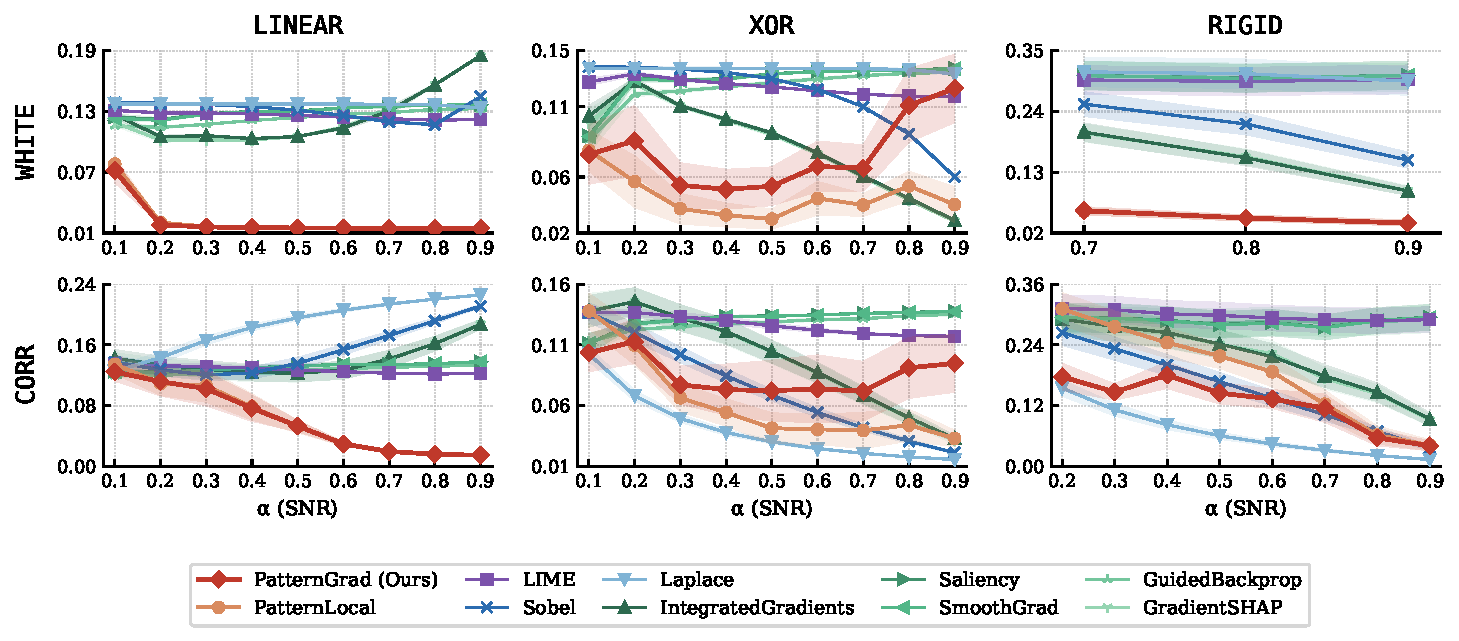
\includegraphics[width=\textwidth]{fig_emd_curves.pdf}
\caption{Earth Mover's Distance (EMD) between the normalized attribution map and the ground-truth support $\mathcal{F}^+$ as a function of the signal-to-noise ratio $\alpha$, for the six XAI-TRIS benchmark suites (columns: \texttt{LIN}, \texttt{XOR}, \texttt{RIGID}; rows: \texttt{WHITE} top, \texttt{CORR} bottom). Shaded bands denote $\pm 1$ standard deviation across the $570$ evaluated held-out instances per configuration; $\alpha$ values removed by the accuracy gate are absent (RIGID-WHITE $\alpha \le 0.6$, RIGID-CORR $\alpha = 0.1$). Lower is better.}
\label{fig:emd_curves}
\end{figure}

\textbf{Linear scenarios.} In LIN-CORR, PatternGrad descends from an EMD of $0.125$ at $\alpha = 0.1$ (rank 3 of 12) to $0.0149$ at $\alpha = 0.9$, where it attains outright rank 1 on both metrics (IME $0.0194$, Sect.~\ref{sec:res_ime}); from $\alpha = 0.7$ onward it recovers the ground-truth support almost exactly, matching PatternLocal to three significant digits ($0.0149$ at $\alpha = 0.9$). In LIN-WHITE the analytic conversion reaches the same recovery floor ($\mathrm{EMD} \approx 0.0147$) by $\alpha = 0.4$ and holds rank 1 of 12 on both metrics from $\alpha = 0.4$ to $0.9$. By contrast, LIME plateaus near $0.12$--$0.13$ across the entire sweep, and the Laplace filter degrades monotonically under correlated noise ($0.125 \to 0.226$ EMD, rank 12 of 12 from $\alpha = 0.2$), confirming that fixed edge operators cannot track the signal statistics as the SNR increases.

\textbf{Rigid-transformation scenarios.} RIGID is the regime that separates the covariance-converted family from both the perturbation surrogates and the raw gradients. In RIGID-CORR, PatternGrad is the only non-filter method ranked in the top two at six of the eight evaluated SNR levels (rank 2 at $\alpha = 0.2$--$0.6$ and $0.8$; rank 3 at $\alpha = 0.9$ with $0.0409$; rank 4 at $\alpha = 0.7$), improving from $0.177$ EMD at $\alpha = 0.2$ to $0.057$ at $\alpha = 0.8$. The Laplace filter is the outright EMD leader at every RIGID-CORR point ($0.155 \to 0.014$), the filter-success effect also observed by Clark et al.~\cite{clark2024}, while PatternLocal trails at ranks 4--5 from $\alpha = 0.4$ onward and LIME stagnates near $0.29$ (rank 9--12). In RIGID-WHITE, where the gate restricts evaluation to $\alpha \ge 0.7$, PatternGrad reaches rank 1 at $\alpha = 0.9$ ($\mathrm{EMD} = 0.0381$, marginally ahead of PatternLocal at $0.0386$). These results show that combining a path-integrated surrogate with training-anchored covariance conversion preserves pixel-level localization under translation and rotation, where conventional attribution maps smear across the position-ambiguous background.

\textbf{XOR scenarios.} XOR is the least favorable regime for PatternGrad in EMD terms. PatternLocal is the outright EMD leader on XOR-WHITE at $\alpha = 0.2$--$0.7$ (its only outright EMD scenario), while PatternGrad holds rank 3 at moderate SNR ($0.051$--$0.054$ at $\alpha = 0.4$--$0.5$) but slips to rank 8 at high SNR ($\mathrm{EMD} = 0.1231$ at $\alpha = 0.9$), an elevated EMD that reflects an intra-support mass imbalance between the two disjoint tetrominoes rather than off-support leakage (Sect.~\ref{sec:res_ablation}). At the highest SNRs the field bunches at the metric floor: on XOR-WHITE at $\alpha = 0.9$, DeepLIFT and GradientSHAP reach $0.0284$ and plain IG $0.0291$, yet all of these maps carry $14$--$15\%$ of their importance mass outside the ground-truth support (IME $\approx 0.147$), whereas the pattern-converted methods concentrate within $1.7\%$ (Sect.~\ref{sec:res_ime}). In XOR-CORR, the Laplace and Sobel filters take the EMD lead at $\alpha = 0.9$ ($0.0157$ and $0.0213$) with PatternGrad at rank 8 ($0.0949$).

\subsection{False-Positive Suppression: IME-Based Results}\label{sec:res_ime}

Figure~\ref{fig:ime_curves} reports the corresponding IME curves, which quantify the fraction of attribution magnitude falling outside $\mathcal{F}^{+}$.

\begin{figure}[t]
\centering
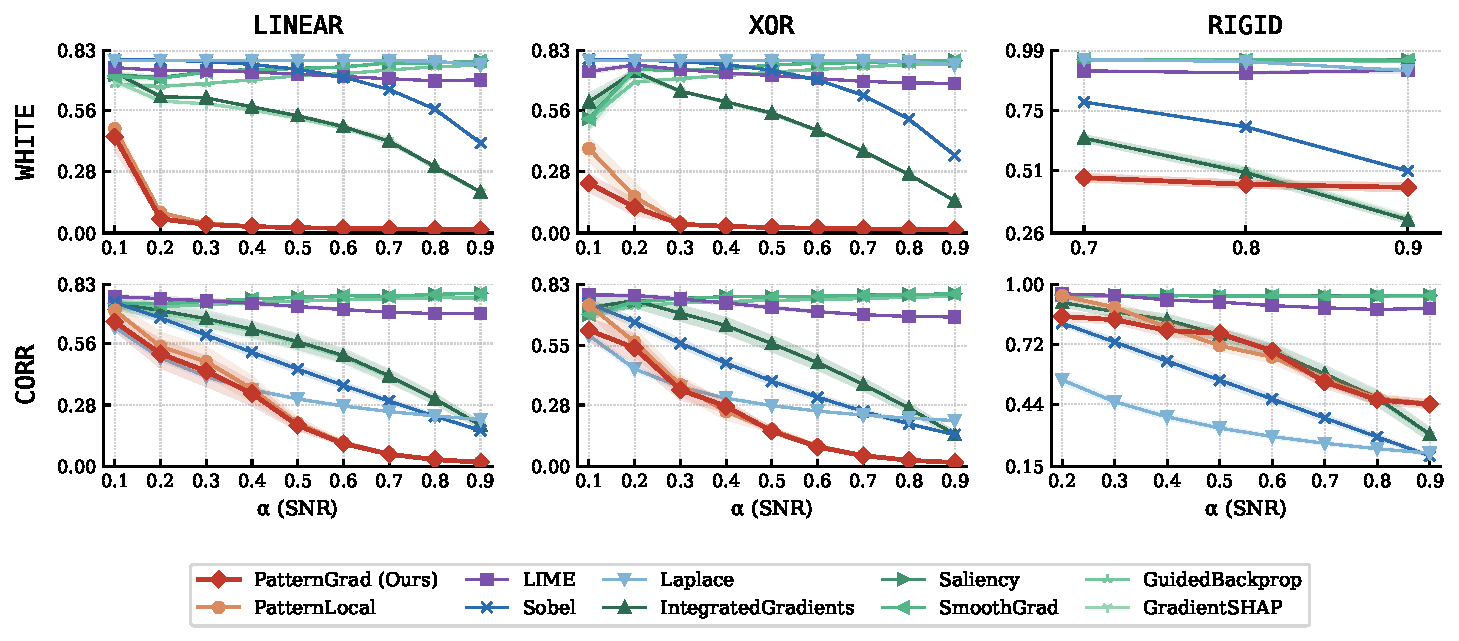
\includegraphics[width=\textwidth]{fig_ime_curves.pdf}
\caption{Importance Mass Error (IME), the fraction of total attribution magnitude placed outside the ground-truth support $\mathcal{F}^{+}$, as a function of the signal-to-noise ratio $\alpha$ (layout and bands as in Fig.~\ref{fig:emd_curves}). Lower is better.}
\label{fig:ime_curves}
\end{figure}

Across the 47 evaluated configurations, PatternGrad ranks in the top three of 12 on IME at 42 configurations and in the top two at 30, and it is the outright IME leader at twelve of them (LIN-WHITE $\alpha = 0.3$--$0.9$, XOR-WHITE $\alpha = 0.3$--$0.5$, LIN-CORR $\alpha = 0.9$, and RIGID-WHITE $\alpha = 0.8$). The five exceptions all occur in the RIGID scenarios at moderate-to-high SNR, where the small, randomly displaced support makes background suppression difficult for every method, and the methods that overtake PatternGrad differ by regime: at RIGID-CORR $\alpha = 0.5$ and $0.6$ the Sobel and Laplace filters lead, with PatternLocal, DeepLIFT, and the IG-family maps also ahead of PatternGrad; at RIGID-CORR $\alpha = 0.8$ and $0.9$ the filters and DeepLIFT attain the lowest IME (e.g., $0.200$ and $0.212$ for Sobel and Laplace at $\alpha = 0.9$, against $0.440$ for PatternGrad, rank 6 of 12); and at RIGID-WHITE $\alpha = 0.9$ the unconverted IG family attains the lowest IME ($0.313$--$0.317$ for Integrated Gradients, DeepLIFT, and GradientSHAP, against $0.443$ for PatternGrad, rank 4 of 12), where Sobel ($0.509$) and Laplace ($0.910$) instead trail PatternGrad. Even in these five configurations PatternGrad remains mid-field (ranks 4--8 of 12), while the unconverted pixel-intensity baselines place up to $95\%$ of their magnitude in the background ($\mathrm{IME} = 0.945$--$0.947$ for Saliency, SmoothGrad, and GuidedBackprop at RIGID-CORR $\alpha = 0.9$).

The suppressor-driven failure mode of discriminative attributions is most visible under correlated noise. On XOR-CORR, PatternGrad reduces its IME from $0.62$ at $\alpha = 0.1$ to $0.018$ at $\alpha = 0.9$ (rank 2), whereas LIME remains flat at $0.68$--$0.79$ over the entire sweep, a roughly 37-fold IME gap at the highest SNR. The same separation appears in the white-noise scenarios at $\alpha \ge 0.3$: PatternGrad, the analytical-grad ablation, and PatternLocal all converge to $\mathrm{IME} \approx 0.016$ on XOR-WHITE at $\alpha = 0.9$, while the raw-gradient family plateaus at $0.15$ (IG, GradientSHAP, DeepLIFT) or $0.77$--$0.79$ (Saliency, SmoothGrad, GuidedBackprop), and LIME at $0.68$. This is the empirical counterpart of Proposition~\ref{prop:suppression}: once the surrogate response is regressed through the local covariance of the training neighborhood, background directions that do not co-vary with the denoised response receive almost no attribution mass, regardless of whether the underlying discriminative vector exploited them.

\subsection{Comparison with State-of-the-Art Pattern Conversion}\label{sec:res_comparison}

Table~\ref{tab:headline} summarizes both metrics at the highest SNR ($\alpha = 0.9$) for all evaluated scenarios. Two complementary profiles emerge. PatternLocal achieves the best support recovery on the XOR scenarios (EMD $0.040$ on XOR-WHITE versus $0.123$ for PatternGrad), reflecting its perturbation-search design that directly minimizes local surrogate disagreement; the PatternGrad gap on XOR stems from an intra-support mass imbalance between the two disjoint tetrominoes rather than off-support leakage (Sect.~\ref{sec:res_ablation}). PatternGrad, in turn, delivers the best false-positive suppression on the linear scenarios, ties the pattern-conversion floor in the remaining scenarios ($\mathrm{IME} \le 0.019$ on XOR and LIN at $\alpha = 0.9$), and matches or exceeds PatternLocal on EMD in the LIN scenarios (both $0.0147$--$0.0149$) and in RIGID-WHITE ($0.0381$ vs.\ $0.0386$). Both pattern methods dominate every gradient-based baseline on IME in the static LIN and XOR scenarios, and dominate LIME on both metrics in all scenarios except the XOR-WHITE EMD floor at $\alpha = 0.9$ (0.123 versus 0.117 for LIME). In the RIGID scenarios at $\alpha = 0.9$, Integrated Gradients (IME $0.300$--$0.313$) and GradientSHAP ($0.296$--$0.317$) achieve lower IME than PatternGrad ($0.440$--$0.443$) and PatternLocal ($0.443$): the unconverted maps scale the path-averaged sensitivities element-wise by the baseline-relative instance, which suppresses the near-zero background pixels immediately adjacent to the displaced tetromino, so roughly $68$--$70\%$ of their attribution mass falls strictly inside the support; their remaining off-support mass, however, is scattered across distant background pixels, producing substantially higher EMD ($0.092$--$0.097$ versus $0.038$--$0.042$). The pattern methods invert this trade-off: local covariance pooling over the $K = 1{,}800$ training neighbors, whose tetrominoes are randomly translated and rotated relative to $\mathbf{x}_\star$, produces a compact spatial halo immediately surrounding the support boundary, placing about $44\%$ of the mass just outside the tight binary mask ($\mathrm{IME} = 0.440$--$0.443$) while keeping the optimal transport distance small ($\mathrm{EMD} = 0.038$--$0.042$).

\begin{table}[t]
\centering
\caption{EMD / IME at $\alpha = 0.9$ for all twelve distinct evaluated methods (thirteen registered entries; the Saliency baseline is numerically identical to the raw Input Gradient after the magnitude normalization used for scoring, marked $^{\dagger}$); $570$ paired instances per cell, mean over instances. Best displayed value per scenario and metric in bold (methods tied at the displayed three-decimal precision are jointly bolded). PG-Grad denotes the analytical-grad ablation (Sect.~\ref{sec:res_ablation}).}
\label{tab:headline}
\footnotesize
\setlength{\tabcolsep}{2.1pt}
\begin{tabular}{lcccccc}
\toprule
 & \multicolumn{2}{c}{\texttt{LIN}} & \multicolumn{2}{c}{\texttt{XOR}} & \multicolumn{2}{c}{\texttt{RIGID}} \\
\textbf{Method} & WHITE & CORR & WHITE & CORR & WHITE & CORR \\
\midrule
PatternGrad (ours) & \textbf{0.015}/\textbf{0.016} & \textbf{0.015}/\textbf{0.019} & 0.123/\textbf{0.016} & 0.095/\textbf{0.018} & \textbf{0.038}/0.443 & 0.041/0.440 \\
PG-Grad (abl.) & \textbf{0.015}/\textbf{0.016} & 0.016/0.031 & 0.084/\textbf{0.016} & 0.068/\textbf{0.018} & 0.044/0.494 & 0.044/0.485 \\
PatternLocal & \textbf{0.015}/\textbf{0.016} & \textbf{0.015}/0.020 & 0.040/\textbf{0.016} & 0.033/\textbf{0.018} & 0.039/0.443 & 0.042/0.443 \\
LIME & 0.122/0.698 & 0.122/0.697 & 0.117/0.682 & 0.117/0.681 & 0.298/0.912 & 0.290/0.887 \\
Saliency$^{\dagger}$ & 0.137/0.784 & 0.138/0.789 & 0.137/0.785 & 0.138/0.787 & 0.306/0.952 & 0.295/0.947 \\
Integrated Gradients & 0.185/0.187 & 0.187/0.188 & 0.029/0.147 & 0.033/0.147 & 0.096/\textbf{0.313} & 0.094/0.300 \\
SmoothGrad & 0.137/0.784 & 0.138/0.789 & 0.137/0.785 & 0.138/0.786 & 0.305/0.952 & 0.294/0.947 \\
DeepLIFT & 0.182/0.193 & 0.187/0.192 & \textbf{0.028}/0.148 & 0.031/0.149 & 0.096/0.316 & 0.088/0.288 \\
GradientSHAP & 0.185/0.187 & 0.188/0.189 & \textbf{0.028}/0.147 & 0.031/0.147 & 0.097/0.317 & 0.092/0.296 \\
GuidedBackprop & 0.133/0.764 & 0.133/0.766 & 0.135/0.771 & 0.135/0.774 & 0.301/0.948 & 0.291/0.945 \\
Sobel & 0.145/0.410 & 0.211/0.164 & 0.060/0.353 & 0.021/0.144 & 0.152/0.509 & 0.036/\textbf{0.200} \\
Laplace & 0.134/0.766 & 0.226/0.214 & 0.133/0.765 & \textbf{0.016}/0.209 & 0.295/0.910 & \textbf{0.014}/0.212 \\
\bottomrule
\end{tabular}
\end{table}

The comparison also highlights a structural asymmetry between the two pipelines, which should be attributed carefully. In the conversion-stage accounting of Table~\ref{tab:runtime}, PatternGrad's speed advantage stems from its matrix-free two-pass evaluation of the closed form over the retrieved neighborhood, against the per-instance weighted regression and neighborhood matrix that PatternLocal's conversion materializes; the elimination of the stochastic surrogate stage itself ($N_{\mathcal{L}} = 2{,}000$ masked forward passes and a local regression per target instance; Sect.~\ref{sec:param_config}) lies outside that accounting and enters only the end-to-end estimates of Sect.~\ref{sec:res_runtime}. With this caveat, PatternGrad attains statistically lower IME than PatternLocal at $\alpha = 0.9$ in four of the six scenarios (LIN-WHITE, LIN-CORR, and XOR-CORR at Holm-adjusted $p < 0.0001$; RIGID-CORR at $p = 0.0056$), a statistical tie in RIGID-WHITE ($p = 0.24$), and a PatternLocal advantage in per-sample IME rank sum on XOR-WHITE ($r = -0.38$, $p < 0.0001$) despite the matching mean IME of $0.016$; it is statistically superior on EMD against the four tested baselines in the LIN and RIGID scenarios (Sect.~\ref{sec:res_stats}; the Sobel and Laplace filters, which are not part of those paired tests, retain lower EMD on RIGID-CORR).

\subsection{Ablation Study: Path Integration versus Raw Input Gradients}\label{sec:res_ablation}

The analytical-grad variant (PG-Grad) applies the identical covariance-conversion pipeline but substitutes the raw input gradient $\nabla_{\mathbf{x}} f(\mathbf{x}_\star)$, the unscaled pointwise local slope, for the IG surrogate $\mathbf{w}^{\text{PG}}$. Because both variants share the kernel, bandwidth, and closed-form estimator of Eq.~\eqref{eq:pg_closed}, any quality difference is attributable to the surrogate choice; note, however, that the two design axes involved, path integration and element-wise instance scaling by $(\mathbf{x}_\star - \mathbf{r})$, are changed simultaneously (Remark~\ref{rem:scaling}). For the near-linear LIN configurations the path integral is nearly exact ($\bar{\mathbf{g}} \approx \nabla_{\mathbf{x}} f$), so there the ablation approximately isolates the instance-scaling choice; for the non-linear scenarios it conflates the two axes.

The ablation separates the two surrogates most sharply in the rigid-transformation scenarios (Table~\ref{tab:headline}). At RIGID-CORR $\alpha = 0.2$, the raw-gradient surrogate collapses to an EMD of $0.291$ (rank 12 of 12) while the path-integrated, instance-scaled surrogate attains $0.177$ (rank 2); the gap persists through moderate SNR ($0.257$ vs.\ $0.181$ at $\alpha = 0.4$, ranks 6 vs.\ 2) and narrows at $\alpha \ge 0.7$, where both converge with the field ($0.044$ vs.\ $0.041$ at $\alpha = 0.9$). Raw gradients are dominated by saturated, spatially diffuse sensitivities once the support moves; the path integral accumulates gradient evidence along the interpolation path and keeps the surrogate response aligned with features that co-vary with the class signal, which is precisely the input that the covariance conversion needs to remain informative (Sect.~\ref{sec:proposed}). Because the two variants differ simultaneously in path integration and in instance scaling, this ablation identifies the combined surrogate design rather than its components separately; an orthogonal $2 \times 2$ design (unscaled path-integrated slope $\bar{\mathbf{g}}$, and instance-scaled pointwise gradient) would isolate the two factors and is left to future work.

Outside the RIGID regime the two variants are closer, with instructive exceptions. In LIN both variants reach the same recovery floor ($0.0147$--$0.016$ EMD at $\alpha \ge 0.4$), and PG-Grad is better at low $\alpha$ (e.g., EMD $0.058$ vs.\ $0.112$ at LIN-CORR $\alpha = 0.2$), where the static support makes the local gradient already informative and path integration adds smoothing cost. This ordering is consistent with the exact-cancellation analysis of Remark~\ref{rem:scaling}: the unscaled slope cancels the suppressor covariance exactly, whereas the instance-scaled surrogate leaves a residual proportional to the target's signal amplitude, which is most visible at low SNR where support recovery is weakest for both variants; the residual becomes negligible relative to the recovery floor as the SNR increases, where the two variants coincide. On XOR at high SNR, PG-Grad is better than PatternGrad on both metrics (XOR-CORR $\alpha = 0.9$: EMD $0.068$ vs.\ $0.095$, IME $0.0178$ vs.\ $0.0183$), but the elevated EMD of the converted variants cannot be explained by the path integral spreading mass onto off-support pixels: the unconverted IG map shares the identical straight-line path integral yet attains EMD $0.029$--$0.033$ on XOR at $\alpha = 0.9$, and both converted variants sit at the IME floor ($0.016$--$0.018$), meaning that more than $98\%$ of their attribution magnitude lies strictly inside $\mathcal{F}^{+}$ and essentially none of it leaks onto the background. The elevated XOR EMD is instead driven by an imbalance of attribution mass between the two spatially disjoint tetrominoes that constitute the support: the T shape occupies the upper-left corner and the L shape the lower-right corner, and each instance realizes one of the four equally likely polarity combinations $\pm\mathbf{a}^{\text{T}} \pm \mathbf{a}^{\text{L}}$ (global sign flips of $\mathbf{a}^{\text{T}} + \mathbf{a}^{\text{L}}$ and $\mathbf{a}^{\text{T}} - \mathbf{a}^{\text{L}}$; Sect.~\ref{sec:dataset}). In the archived per-instance attribution maps for XOR-WHITE $\alpha = 0.9$, the T-to-L mass split of PatternGrad ranges from $0.5$ to $6.2$ across the five saved instances, with the dominant direction varying from instance to instance; the optimal transport plan must then carry the surplus mass across the image diagonal from one tetromino to the other, inflating EMD while IME remains at the floor. The neighborhood used on XOR at $\alpha \ge 0.4$ is the global one ($K = 36{,}000 = N_{\text{train}}$, Table~\ref{tab:k_selection}), reached because PatternLocal's $k_{\text{ratio}}$ search selected $k_{\text{ratio}} = 1.0$ under the same mean-EMD tuning objective on the $30$-instance tuning subset, so PatternGrad's floor-coupled candidate grid collapsed to the single candidate $K = N_{\text{train}}$ (Sect.~\ref{sec:hyper}); pooling across all four polarity sub-clusters, between which the two tetrominoes are globally uncorrelated, yields a covariance $\mathbf{C}_K$ that does not couple the two supports and therefore cannot rebalance an asymmetry present in the surrogate vector. This residual cost is shared by both converted variants, while PatternLocal's LIME-derived surrogate avoids it. Overall, the instance-scaled, path-integrated surrogate buys robustness to geometric variance, at the price of a residual cost that vanishes at high SNR on the linear tasks but persists on XOR as the intra-support imbalance described above.

\subsection{Statistical Analysis}\label{sec:res_stats}

Table~\ref{tab:wilcoxon} reports paired two-sided Wilcoxon signed-rank tests~\cite{wilcoxon1945} between PatternGrad and PatternLocal, LIME, plain IG, and the PG-Grad ablation on the $570$ per-sample EMD and IME scores at $\alpha = 0.9$, with Holm correction across the four comparisons per cell and rank-biserial correlation $r$ as the effect size.

\begin{table}[t]
\centering
\caption{Paired two-sided Wilcoxon signed-rank tests comparing PatternGrad against the leading baselines on per-sample EMD and IME at high signal-to-noise ratio ($\alpha$ = 0.9; $570$ paired instances per cell). $p$-values are Holm-corrected across the four comparisons per cell; $r$ is the rank-biserial effect size (positive $r$: PatternGrad attains the lower error, negative $r$: the baseline does), and $\widetilde{\Delta}$ is the median of the paired per-sample differences (PatternGrad minus baseline; negative values favor PatternGrad). $W$ is the smaller of the two rank sums, so $W = 0$ with $|r| = 1$ indicates complete pairwise dominance by one method; at the metric floors, significant $r$ values can coexist with median differences that are zero to three decimals.}
\footnotesize
\setlength{\tabcolsep}{2.6pt}
\label{tab:wilcoxon}
\begin{tabular}{ll rrrr rrrr}
\toprule
& & \multicolumn{4}{c}{EMD} & \multicolumn{4}{c}{IME}\\
\cmidrule(lr){3-6}\cmidrule(lr){7-10}
\textbf{Scenario} & \textbf{Baseline} & $W$ & $p$ & $r$ & $\widetilde{\Delta}$ & $W$ & $p$ & $r$ & $\widetilde{\Delta}$\\
\midrule
LIN-WHITE & PatternLocal & 33277 & $<$0.0001 & +0.59 & -0.0000 & 2901 & $<$0.0001 & +0.96 & -0.0000 \\
LIN-WHITE & LIME & 0 & $<$0.0001 & +1.00 & -0.1074 & 0 & $<$0.0001 & +1.00 & -0.6810 \\
LIN-WHITE & IG & 0 & $<$0.0001 & +1.00 & -0.1704 & 0 & $<$0.0001 & +1.00 & -0.1712 \\
LIN-WHITE & PG-Grad (abl.) & 42195 & $<$0.0001 & +0.48 & +0.0000 & 0 & $<$0.0001 & +1.00 & -0.0000 \\
\addlinespace
LIN-CORR & PatternLocal & 49697 & $<$0.0001 & +0.39 & -0.0000 & 47688 & $<$0.0001 & +0.41 & -0.0003 \\
LIN-CORR & LIME & 0 & $<$0.0001 & +1.00 & -0.1075 & 0 & $<$0.0001 & +1.00 & -0.6777 \\
LIN-CORR & IG & 0 & $<$0.0001 & +1.00 & -0.1738 & 0 & $<$0.0001 & +1.00 & -0.1672 \\
LIN-CORR & PG-Grad (abl.) & 42135 & $<$0.0001 & +0.48 & -0.0000 & 40008 & $<$0.0001 & +0.51 & -0.0020 \\
\addlinespace
XOR-WHITE & PatternLocal & 0 & $<$0.0001 & -1.00 & +0.0828 & 50142 & $<$0.0001 & -0.38 & +0.0000 \\
XOR-WHITE & LIME & 76939 & 0.2602 & -0.05 & -0.0031 & 0 & $<$0.0001 & +1.00 & -0.6649 \\
XOR-WHITE & IG & 3 & $<$0.0001 & -1.00 & +0.0850 & 0 & $<$0.0001 & +1.00 & -0.1306 \\
XOR-WHITE & PG-Grad (abl.) & 2218 & $<$0.0001 & -0.97 & +0.0409 & 43601 & $<$0.0001 & -0.46 & +0.0001 \\
\addlinespace
XOR-CORR & PatternLocal & 939 & $<$0.0001 & -0.99 & +0.0497 & 59662 & $<$0.0001 & +0.27 & -0.0001 \\
XOR-CORR & LIME & 41092 & $<$0.0001 & +0.49 & -0.0329 & 0 & $<$0.0001 & +1.00 & -0.6621 \\
XOR-CORR & IG & 2276 & $<$0.0001 & -0.97 & +0.0520 & 0 & $<$0.0001 & +1.00 & -0.1256 \\
XOR-CORR & PG-Grad (abl.) & 12310 & $<$0.0001 & -0.85 & +0.0237 & 31920 & $<$0.0001 & -0.61 & +0.0007 \\
\addlinespace
RIGID-WHITE & PatternLocal & 66055 & 0.0002 & +0.19 & -0.0004 & 76702 & 0.2356 & +0.06 & -0.0009 \\
RIGID-WHITE & LIME & 0 & $<$0.0001 & +1.00 & -0.2630 & 0 & $<$0.0001 & +1.00 & -0.4716 \\
RIGID-WHITE & IG & 21 & $<$0.0001 & +1.00 & -0.0583 & 9 & $<$0.0001 & -1.00 & +0.1221 \\
RIGID-WHITE & PG-Grad (abl.) & 16937 & $<$0.0001 & +0.79 & -0.0057 & 11877 & $<$0.0001 & +0.85 & -0.0482 \\
\addlinespace
RIGID-CORR & PatternLocal & 70190 & 0.0056 & +0.14 & -0.0004 & 69601 & 0.0056 & +0.14 & -0.0017 \\
RIGID-CORR & LIME & 0 & $<$0.0001 & +1.00 & -0.2525 & 0 & $<$0.0001 & +1.00 & -0.4480 \\
RIGID-CORR & IG & 1876 & $<$0.0001 & +0.98 & -0.0507 & 1546 & $<$0.0001 & -0.98 & +0.1447 \\
RIGID-CORR & PG-Grad (abl.) & 39066 & $<$0.0001 & +0.52 & -0.0029 & 18017 & $<$0.0001 & +0.78 & -0.0311 \\
\bottomrule
\end{tabular}
\end{table}

The tests confirm the visual reading of Figs.~\ref{fig:emd_curves} and \ref{fig:ime_curves}. Twenty-two of the 24 comparisons are significant after Holm correction at the $0.05$ level (all but the XOR-WHITE EMD comparison against LIME, $p = 0.26$, where PatternGrad and LIME plateau near $0.123$ and $0.117$, well above the $0.028$--$0.040$ floor that GradientSHAP, plain IG, and PatternLocal reach on that scenario, and the RIGID-WHITE IME comparison against PatternLocal, $p = 0.24$, where the two pattern methods tie at $0.443$, well above plain IG's $0.313$ and the theoretical floor of $0$). The effect sizes separate the scenarios cleanly: on both LIN scenarios PatternGrad holds large positive effects against all baselines ($r$ up to $+1.00$, complete pairwise dominance against LIME and IG), on the XOR scenarios the effect reverses against PatternLocal on EMD ($r = -0.99$ to $-1.00$) but stays positive against LIME on IME and against the raw-gradient baselines, and on the RIGID scenarios PatternGrad retains a positive EMD effect against PatternLocal ($r = +0.14$ to $+0.19$) and a large positive effect against the ablation ($r = +0.52$ to $+0.85$). The only reversals against non-ablation baselines are the EMD effect of PatternLocal in XOR (expected from Fig.~\ref{fig:emd_curves}) and the IME effect of plain IG in RIGID ($r = -1.00$ and $-0.98$), consistent with the halo-versus-scatter mass-positioning profile discussed in Sect.~\ref{sec:res_comparison}. The median paired differences $\widetilde{\Delta}$ in Table~\ref{tab:wilcoxon} separate effect magnitude from effect consistency: several significant comparisons sit at the metric floors, where per-instance differences are microscopic even when they are one-sided. On the LIN recovery floor, the medians against PatternLocal are $-0.0000$ in EMD and $-0.0000$ to $-0.0003$ in IME (that is, below $10^{-3}$ in absolute value on every such cell), and against the PG-Grad ablation they are $\pm 0.0000$ in EMD; on the XOR pattern-conversion IME floor the medians against PatternLocal are $+0.0000$ to $-0.0001$; and in the RIGID-WHITE IME tie against PatternLocal the median is $-0.0009$, with the tie decided by ranking rather than by magnitude. Where the medians are large and one-sided, the comparisons are practically as well as statistically meaningful (for example, the IME advantage over LIME on LIN, median $-0.68$, and the XOR EMD advantage of PatternLocal over PatternGrad, median $+0.05$ to $+0.08$).

\subsection{Runtime Comparison}\label{sec:res_runtime}

Table~\ref{tab:runtime} reports the per-sample wall-clock cost of the conversion stage, measured on single-vCPU instances (Sect.~\ref{sec:repro}). The timed region comprises the kernel weighting, the bandwidth computation, and the $\mathcal{O}(KD)$ two-pass covariance product of Algorithm~\ref{algo:patterngrad} (lines 3--6), plus map normalization. The per-instance IG surrogate ($M = 50$ backward passes) and the exact Euclidean $K$-nearest-neighbor retrieval over $\mathcal{D}_{\text{train}}$ (Algorithm~\ref{algo:patterngrad}, line 2, $\mathcal{O}(ND)$) are computed once per instance outside the timed region and shared across all evaluated methods and candidate neighborhoods (the retrieval is executed with the full neighbor list, from which every candidate neighborhood is a prefix slice), so the reported times exclude the retrieval and surrogate terms of the per-instance complexity accounting in Sect.~\ref{sec:proposed}. PatternLocal's measured time likewise covers only its conversion stage, the neighborhood-weighted covariance of Eq.~\eqref{eq:pl_closed} applied to the precomputed LIME explanation, so Table~\ref{tab:runtime} compares the two conversion stages under identical accounting; the LIME front-end ($N_{\mathcal{L}} = 2{,}000$ masked forward passes plus a weighted ridge fit over the pixel-level $D' = D = 4{,}096$ mask space; Sect.~\ref{sec:param_config}) is PatternLocal's own surrogate stage and is excluded from its reported time. To quantify the full measured pipeline, we additionally account the per-instance IG surrogate front-end, the $M = 50$ backward-pass loop, timed under the identical accounting as the unconverted plain IG baseline: $0.094$--$0.161$~s per instance (median $0.141$~s) across the $47$ evaluated configurations. PatternGrad's end-to-end measured pipeline (surrogate plus conversion, still excluding the shared nearest-neighbor retrieval) is therefore $0.102$--$0.316$~s per explained instance (median $0.212$~s). Even on this deliberately conservative comparison, in which PatternLocal is charged only its conversion stage, PatternGrad's measured pipeline is faster in all $47$ configurations ($1.8\times$--$5.0\times$, median $3.2\times$), and the LIME front-end, which the sweeps did not instrument separately, would only add to PatternLocal's end-to-end cost. In conversion-stage terms, PatternGrad required between $0.007$ and $0.173$ seconds per explained instance (median $0.074$), against $0.40$--$0.80$ seconds (median $0.69$) for PatternLocal, yielding per-configuration conversion-stage speedups between $3.4\times$ and $81.8\times$ (median $9.2\times$); PatternLocal's conversion cost is nearly independent of the scenario.

The spread within PatternGrad is not monotone in $K$ because the implementation distinguishes two branches of the covariance product. When the selected neighborhood equals the full training set ($K = N_{\text{train}} = 36{,}000$, as in all white-noise configurations and the high-SNR correlated-noise points), the kernel weights are scattered into a length-$N$ vector and the two-pass product runs directly on the contiguous, pre-stored float32 training matrix, so no per-instance neighborhood copy is made. When $K < N_{\text{train}}$, a fresh $K \times D$ neighborhood matrix is materialized per instance by a random-access gather from the training matrix (about $327$~MB at $K = 20{,}000$, $D = 4{,}096$, float32), and this cache-hostile copy, not the $\mathcal{O}(KD)$ product, dominates the measured time. This explains the counterintuitive ordering in Table~\ref{tab:runtime} combined with Table~\ref{tab:k_selection}: LIN-WHITE and XOR-WHITE, which select $K = 36{,}000$ at every $\alpha$, run in $0.063$--$0.089$~s, whereas the slowest configuration, LIN-CORR $\alpha = 0.4$ with the smaller $K = 20{,}000$, takes $0.173$~s; the small-neighborhood configurations ($K = 1{,}800$: all RIGID-WHITE and RIGID-CORR points at $\alpha \ge 0.7$ and the low-$\alpha$ CORR points) gather only about $30$~MB and run in $0.007$--$0.011$~s at $56$--$82\times$ speedup.

\begin{table}[t]
\centering
\caption{Per-sample conversion-stage runtime (seconds per explained instance) over the evaluated configurations of each scenario, measured on single-vCPU instances. Times cover Algorithm~\ref{algo:patterngrad} lines 3--6 for PatternGrad and the corresponding neighborhood-covariance stage of Eq.~\eqref{eq:pl_closed} for PatternLocal; the per-instance surrogate front-ends ($M = 50$ IG backward passes; the LIME fit with $N_{\mathcal{L}} = 2{,}000$ perturbation samples over the pixel-level $D' = D = 4{,}096$ mask space) and the exact Euclidean $K$-nearest-neighbor retrieval ($\mathcal{O}(ND)$) are computed once per instance outside the timed region and shared across all methods (Sect.~\ref{sec:res_runtime}). Speedup is PatternLocal's per-configuration time divided by PatternGrad's.}
\label{tab:runtime}
\begin{tabular}{lccc}
\toprule
\textbf{Scenario} & \textbf{PatternGrad (s)} & \textbf{PatternLocal (s)} & \textbf{Speedup ($\times$)} \\
\midrule
LIN-WHITE  & 0.063--0.089 & 0.558--0.804 & 7.5--11.2 \\
LIN-CORR   & 0.011--0.173 & 0.476--0.795 & 3.4--68.2 \\
XOR-WHITE  & 0.063--0.078 & 0.582--0.722 & 7.6--11.0 \\
XOR-CORR   & 0.007--0.145 & 0.404--0.787 & 5.0--59.5 \\
RIGID-WHITE & 0.009--0.011 & 0.723--0.760 & 64.9--81.8 \\
RIGID-CORR & 0.007--0.159 & 0.404--0.745 & 4.3--65.8 \\
\midrule
All configurations & 0.007--0.173 & 0.404--0.804 & 3.4--81.8 (median 9.2) \\
\bottomrule
\end{tabular}
\end{table}

\subsection{Qualitative Analysis}\label{sec:res_qualitative}

Figure~\ref{fig:qualitative} displays signed attribution maps for six representative conditions spanning both noise regimes and all three tasks.

\begin{figure}[t]
\centering
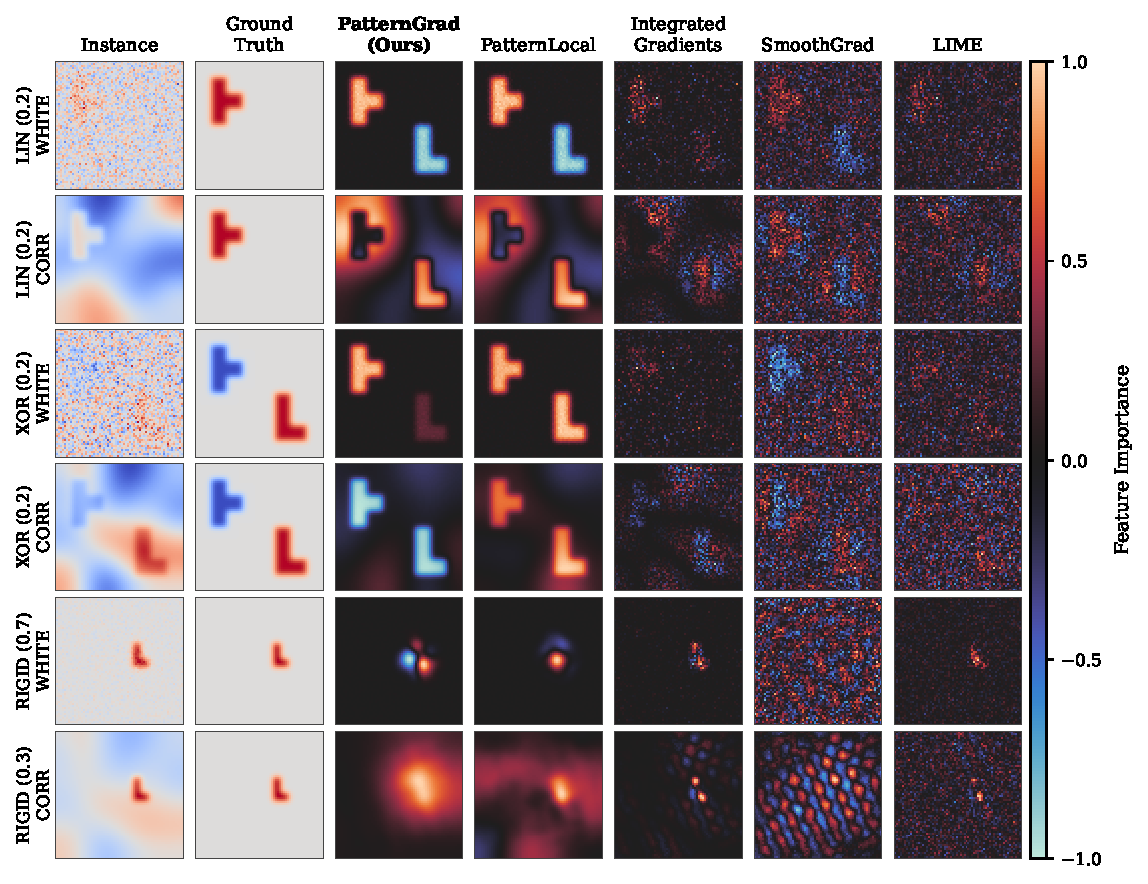
\includegraphics[width=\textwidth]{fig_qualitative.pdf}
\caption{Qualitative comparison on held-out test instances. Rows (top to bottom): LIN-WHITE $\alpha=0.2$, LIN-CORR $\alpha=0.2$, XOR-WHITE $\alpha=0.2$, XOR-CORR $\alpha=0.2$, RIGID-WHITE $\alpha=0.7$, RIGID-CORR $\alpha=0.3$. Columns: input instance, ground-truth support $\mathcal{F}^{+}$, and the signed attribution maps of PatternGrad, PatternLocal, Integrated Gradients, SmoothGrad, and LIME, all after identical max-magnitude normalization on the shared color scale $[-1, 1]$.}
\label{fig:qualitative}
\end{figure}

The maps make the mechanism behind the quantitative results visible. In the LIN rows, PatternGrad and PatternLocal both reproduce the two tetromino supports with the correct signed contrast (positive on the class-bearing shape, negative on the complementary shape), while Integrated Gradients, SmoothGrad, and LIME scatter low-amplitude importance across the entire background, exactly the suppressor leakage that IME penalizes. In the XOR rows, where the two shapes carry opposite polarity within each class, PatternGrad preserves the relative polarity of the two tetrominoes on both WHITE and CORR backgrounds; under correlated noise the two pattern methods additionally reproduce the smooth background perturbation shell that the classifier uses for denoising, but only outside the support does their mass decay, whereas the gradient baselines highlight the noise texture itself. In the RIGID rows, PatternGrad localizes a compact positive region around the displaced tetromino despite its arbitrary position and orientation, PatternLocal exhibits a similar concentration with a broader halo, SmoothGrad produces a periodic interference pattern, and LIME stays near its noise floor. Together with the EMD and IME curves, this confirms that the qualitative behavior of PatternGrad (concentration on the informative support, suppression of uncorrelated background, and robustness to spatial displacement) matches the statistical aggregates rather than holding only for cherry-picked instances.

\subsection{Key Findings and Discussion}\label{sec:res_findings}

The evaluation supports five principal findings.

\begin{enumerate}
    \item \textbf{Covariance conversion removes suppressor-induced false positives.} PatternGrad ranks in the top three of 12 methods on IME at 42 of 47 configurations and is the outright IME leader at twelve, reducing off-support mass to $1.6$--$1.9\%$ in the static LIN and XOR scenarios at high SNR, where unconverted gradient and perturbation baselines leave $15$--$79\%$ of their importance mass in the background; in the RIGID scenarios the neighborhood halo (Sect.~\ref{sec:res_comparison}) keeps PatternGrad at $44.0$--$44.3\%$, above the unconverted IG family (Integrated Gradients $30.0$--$31.3\%$, GradientSHAP $29.6$--$31.7\%$) but still far below the pixel-intensity baselines ($94$--$95\%$). This is the empirical signature of the suppressor-cancellation mechanism formalized in Proposition~\ref{prop:suppression}.
    \item \textbf{PatternGrad and PatternLocal are complementary rather than interchangeable.} PatternLocal attains the best support recovery (EMD) on the XOR scenarios, PatternGrad attains the best false-positive suppression (IME) on the linear scenarios and the best EMD on the linear and RIGID-WHITE scenarios, and the two are statistically indistinguishable in the RIGID-WHITE IME tie at $0.443$. Neither method dominates the field on both metrics, so the choice between them is governed by which error type matters for the application.
    \item \textbf{The path-integrated, instance-scaled surrogate survives geometric transformation.} Replacing the IG surrogate with the raw input gradient in the identical pipeline collapses RIGID-CORR EMD from rank 2 to rank 12 (of 12 distinct methods) at low SNR, while both variants remain at the recovery floor in the static scenarios. The combined path-integrated, instance-scaled surrogate design is therefore the component responsible for robustness under translation and rotation within this pipeline; because the ablation introduces path integration and instance scaling together, attribution to the individual factors (unscaled path-integrated slope, or scaled pointwise gradient) was not tested and is left to future work, and the unscaled slope remains the stronger surrogate in the linear scenarios at low SNR, consistent with its exact suppressor cancellation (Remark~\ref{rem:scaling}).
    \item \textbf{Deterministic conversion is substantially cheaper end-to-end.} Under the shared accounting of Sect.~\ref{sec:res_runtime}, PatternGrad's conversion stage takes $0.007$--$0.173$~s per sample (median $0.074$~s) on a single CPU, $3.4\times$ to $81.8\times$ faster than PatternLocal's (median $9.2\times$; conversion-stage accounting). Adding the measured $M = 50$-backward-pass surrogate front-end, PatternGrad's full measured pipeline is $0.102$--$0.316$~s per explained instance (median $0.212$~s), which remains below PatternLocal's conversion stage alone ($0.404$--$0.804$~s) in all $47$ configurations ($1.8\times$--$5.0\times$, median $3.2\times$); PatternLocal's stochastic LIME front-end was not instrumented separately and would only add to its end-to-end cost. The conversion-stage margins are largest exactly where explanations must scale, in the high-SNR RIGID regimes.
    \item \textbf{Known limitations.} PatternGrad's EMD weakens on the XOR scenarios at high SNR (rank 8 of 12 at $\alpha = 0.9$), where sign-alternating polarity induces an intra-support mass imbalance between the two disjoint tetrominoes under the global covariance neighborhood (Sect.~\ref{sec:res_ablation}) and metric-floor bunching favors PatternLocal and several gradient methods; its IME in the RIGID scenarios remains elevated ($0.440$--$0.443$), exceeded there by the unconverted IG family on both RIGID scenarios (Integrated Gradients $0.300$--$0.313$, GradientSHAP $0.296$--$0.317$, DeepLIFT $0.288$--$0.316$ at $\alpha = 0.9$) and by the Sobel and Laplace filters on RIGID-CORR only ($0.200$ and $0.212$; on RIGID-WHITE the filters trail at $0.509$ and $0.910$); the evaluation is confined to the additive scenarios of synthetic XAI-TRIS data (the multiplicative \texttt{MULT} scenario is omitted, Sect.~\ref{sec:dataset}); and the $K$ selected by validation directly trades runtime against locality, with the largest-neighborhood configurations costing up to $0.173$~s per sample in the conversion stage (Sect.~\ref{sec:res_runtime}). A further scope caveat concerns retrieval scalability: the exact Euclidean $K$-nearest-neighbor search operates in raw pixel space at $\mathcal{O}(ND)$ per instance, which at the XAI-TRIS scale ($D = 4{,}096$, $N_{\text{train}} = 36{,}000$) is a single inexpensive pass computed once per instance outside the timed conversion stage and shared across all methods (it is not included in the conversion-stage runtimes of Sect.~\ref{sec:res_runtime}), but in higher-dimensional clinical data (e.g., neuroimaging volumes) exact retrieval would become the computational bottleneck, requiring dimensionality reduction, approximate nearest-neighbor structures, or learned embedding spaces; the covariance conversion itself remains $\mathcal{O}(KD)$. Finally, three protocol extensions that could sharpen the causal picture were designed out of the present sweeps rather than run: a decoupled PatternGrad neighborhood search on the high-SNR \texttt{XOR} configurations (the floor coupling precludes a small uncoupled $K$ there; Sect.~\ref{sec:hyper}), an orthogonal $2 \times 2$ surrogate ablation separating path integration from instance scaling (Sect.~\ref{sec:res_ablation}), and a larger-$N_{\mathcal{L}}$ LIME control probing whether the strongly under-determined pixel-level surrogate fit ($N_{\mathcal{L}} = 2{,}000$ against $D' = 4{,}096$) is itself a source of the baseline's estimation variance.
\end{enumerate}

Taken together, these results substantiate the claims of the abstract with a measured, paired-verification protocol: PatternGrad matches or exceeds state-of-the-art perturbation-based pattern conversion in false-positive suppression and spatial localization wherever the support is linear or displaced, does so deterministically and at pixel resolution without superpixel artifacts, and does so at a fraction of the computational cost.

\section{Conclusion}\label{sec:conclusion}

This paper addressed the tendency of post-hoc attribution methods to assign false-positive importance to suppressor variables, features that carry no class information but correlate with the noise corrupting the informative signal. PatternGrad removes the three practical bottlenecks of perturbation-driven local pattern explanation, namely randomized perturbation sampling, per-instance surrogate fitting, and superpixel discretization, by pairing the deterministic, native-pixel-space attribution vector of Integrated Gradients with the training-anchored covariance conversion of PatternLocal, evaluated in closed form through an $\mathcal{O}(KD)$ matrix-free two-pass product after exact neighbor retrieval. On 47 configurations of the XAI-TRIS benchmark, this design ranks in the top three of the twelve distinct methods on false-positive suppression (IME) at 42 configurations and is the outright leader at twelve, recovers the ground-truth support almost exactly in the linear scenarios ($\mathrm{EMD} \approx 0.015$ at high SNR), and is the only non-filter method in the top two on spatial localization (EMD) at six of the eight evaluated RIGID-CORR points. The method is not uniformly superior: on the XOR scenarios at high SNR its EMD degrades ($0.095$--$0.123$ at $\alpha = 0.9$) because the global covariance neighborhood cannot rebalance attribution mass between the two disjoint tetrominoes, leaving PatternLocal ahead there, and on the RIGID scenarios its IME ($0.440$--$0.443$) is exceeded by the unconverted IG family, reflecting a halo-versus-scatter trade-off in how off-support mass is positioned. The measured pipeline (surrogate plus conversion) runs in $0.10$--$0.32$~s per explained instance on a single CPU, below the conversion stage alone of surrogate-based pattern conversion. Future work includes validation on real-world correlated-noise modalities, polarity-aware surrogate designs for the XOR scenarios, the fully integrated but unscaled surrogate variant with optional post-conversion rescaling (Remark~\ref{rem:scaling}), decoupled neighborhood tuning, adaptive per-instance neighborhood selection, and scaling the covariance conversion to convolutional architectures and higher-resolution inputs.

\backmatter

\bmhead{Acknowledgements}

The authors thank the developers of the XAI-TRIS benchmark and the PatternLocal reference implementation for releasing the data-generation and evaluation code that made this study reproducible.

\bmhead{Author contributions}

Md Arif Faysal Nayem: conceptualization, methodology, software, investigation, formal analysis, visualization, writing (original draft). Ohidujjaman: supervision, validation, writing (review and editing).

\bmhead{Funding}

The authors declare that no funds, grants, or other support were received during the preparation of this manuscript.

\bmhead{Competing interests}

The authors have no relevant financial or non-financial interests to disclose.

\bmhead{Data availability}

The XAI-TRIS benchmark is publicly available from the original authors of the benchmark. The aggregated evaluation outputs (per-sample scores, sweep summaries, and figures) supporting the results of this article are available from the corresponding author upon reasonable request.

\bmhead{Code availability}

The implementation of PatternGrad and the evaluation pipeline used in this study will be made publicly available upon publication.

\bibliography{sn-bibliography}

\end{document}
